%%=============================================
% !Mode:: "TeX:UTF-8"
% !TEX program  = xelatex
%%=============================================
% 哈尔滨工业大学（深圳）硕士学位论文 —— 中期论文初稿
% 课题：基于代理模型的无人机螺旋桨前飞工况气动外形优化
% 作者：郭跃  学号：24S153206  导师：何晓舟 教授
% 学院：机器人与先进制造学院  专业：能源动力
%%=============================================

\documentclass[fontset=fandol,type=master]{hithesisbook}

\usepackage{bm}
\usepackage{booktabs}
\usepackage{array}

\setmainfont{Times New Roman}
\setsansfont{Arial}
\setCJKmainfont{Songti SC}
\setCJKsansfont{Heiti SC}
\setCJKfamilyfont{zhsong}{Songti SC}
\setCJKfamilyfont{zhhei}{Heiti SC}

\makeatletter
\renewcommand\normalsize{%
  \@setfontsize\normalsize{12bp}{15bp}%
  \abovedisplayskip=8pt
  \abovedisplayshortskip=8pt
  \belowdisplayskip=\abovedisplayskip
  \belowdisplayshortskip=\abovedisplayshortskip}
\makeatother
\normalsize

\ctexset{
  section/format={\heiti\xiaosan},
  subsection/format={\heiti\sihao},
  subsubsection/format={\heiti\xiaosi}
}

\AtBeginEnvironment{table}{\wuhao}
\AtBeginEnvironment{longtable}{\wuhao}

\graphicspath{{figures/}}

\begin{document}

% 前置部分
\frontmatter

% !TEX root = ../thesis.tex

\hitsetup{
  %=========
  % 中文信息
  %=========
  ctitle={基于代理模型的无人机螺旋桨前飞工况气动外形优化},
  ctitlecover={基于代理模型的无人机螺旋桨前飞工况气动外形优化},
  ckeywords={螺旋桨气动外形优化; 自由涡尾迹方法; 异方差代理模型; 不确定度量化; CMA-ES; 差速配平嵌套优化},
  cxueke={工学},
  csubject={能源动力},
  caffil={机器人与先进制造学院},
  cauthor={郭跃},
  csupervisor={何晓舟 教授},
  cdate={2026年7月},
  cstudentid={24S153206},
  %=========
  % 英文信息
  %=========
  etitle={Surrogate-Model-Based Aerodynamic Shape Optimization of UAV Propellers under Forward-Flight Condition},
  ekeywords={Propeller aerodynamic optimization, Lifting-Line Free Vortex Wake, Heteroscedastic surrogate model, Uncertainty quantification, CMA-ES, Differential-trim nested optimization},
  exueke={Engineering},
  esubject={Energy and Power Engineering},
  eaffil={School of Mechanical Engineering and Automation},
  eauthor={Yue Guo},
  esupervisor={Prof. Xiaozhou He},
  edate={June 2026}
}

% 中文摘要
\begin{cabstract}

随着低空经济发展，小型无人机在城市低空场景广泛承担巡航、配送等任务，螺旋桨气动外形对推进效率与三轴平衡能力具有决定性作用。本课题针对 X 构型四旋翼无人机前飞工况开展螺旋桨气动外形优化研究：前飞工况包含非轴向来流的尾迹—桨叶耦合、前后桨升力差导致的俯仰矩耦合以及三轴差速配平约束等典型耦合特征，对气动求解效率、代理模型可信度和优化结果物理可实现性提出了更高要求。本文面向前飞巡航效率提升与配平能力保持，建立兼顾计算效率、预测精度和不确定度感知能力的螺旋桨外形优化方法。

围绕上述需求，本文构建了建模、代理预测、优化和高保真验证相结合的螺旋桨气动外形优化平台。在气动建模层面，以 8 个 B-Spline 控制点描述弦长与扭角分布并插值得到 22 个径向截面，结合非线性升力线自由涡尾迹（Lifting-Line Free Vortex Wake, LLFVW）方法构建低成本求解器，并通过翼型层（XFoil, $Re=10^5\sim 3\times 10^5$）和螺旋桨层（APC 10$\times$7, $\text{RPM}\in[4007,6519]$）两级对照 UIUC 风洞数据完成验证。在代理建模层面，采用异方差多层感知机配合 LIFT-NLL 损失，输出推力、面内力、俯仰力矩和扭矩的预测均值 $\mu$ 与不确定度 $\sigma$；在 237 几何 9954 样本上训练，测试集 MAE 为 0.0332、$R^2$ 达到 0.987、俯仰力矩校准误差 ECE 为 0.13，参数量仅 80K，兼顾精度与推理效率。

在优化层面，本文以 CMA-ES 全局优化器结合数据驱动硬约束，并将三轴差速配平求解器嵌入目标函数评估流程，同步求解迎角 $\alpha$ 与前后桨转速 $\Omega_1,\Omega_2$。目标函数综合电功率、配平残差、代理不确定度和几何光顺性，使候选外形在气动性能与物理可实现性之间取得平衡。优化结果在方法学验证集上达到 $FM=0.947$、$P_{\text{elec}}=362.7\,\text{W}$，相比基线 APC 10$\times$7 螺旋桨在推进效率和前飞配平性能上均有显著提升。本文同步建立了 Star-CCM+ CFD 验证模板（$\sim 700$ 万网格、$y^+ \in [0,1]$、SST $k$-$\omega$、误差 $\leq 5\%$）用于优化外形的独立高保真验证。

本文的主要创新成果在于：（1）以 LLFVW 替代高成本 CFD 作为优化内循环求解器，在保持前飞尾迹耦合描述的同时显著降低样本生成成本；（2）通过异方差代理模型同步给出预测值与不确定度，为优化过程提供可信度约束并支撑主动补点闭环；（3）将差速配平作为算子嵌入气动外形优化的目标函数评估，使优化结果在前飞工况下物理可实现。

\end{cabstract}

\begin{eabstract}

With the rapid development of the low-altitude economy, small unmanned aerial vehicles (UAVs) widely undertake cruise and delivery tasks in urban low-altitude scenarios. The propeller, as a critical component of the propulsion system, has a decisive influence on propulsion efficiency and three-axis trim capability. This work addresses propeller aerodynamic shape optimization for X-configuration quadrotor UAVs under steady free-stream forward-flight conditions. Forward flight involves non-axial inflow wake-blade coupling, pitch-moment coupling caused by front-rear thrust differential, and three-axis differential-trim constraints, placing higher requirements on aerodynamic-solver efficiency, surrogate-model credibility, and physical realizability of optimized geometries. Therefore, this study develops a propeller shape optimization method that improves forward-flight cruise efficiency while preserving trim capability, with emphasis on computational efficiency, prediction accuracy, and uncertainty awareness.

This study constructs an integrated platform that combines aerodynamic modeling, surrogate prediction, optimization, and high-fidelity validation. At the geometry and aerodynamic modeling layer, the chord and twist distributions are parameterized by 8 B-Spline control points and interpolated into 22 radial sections. A low-cost aerodynamic solver is established based on the nonlinear Lifting-Line Free Vortex Wake (LLFVW) method and validated against the UIUC wind-tunnel database at both the airfoil level (XFoil, $Re=10^5\sim 3\times 10^5$) and the propeller level (APC 10$\times$7, $\text{RPM}\in[4007,6519]$). At the surrogate modeling layer, a Heteroscedastic MLP trained with LIFT-NLL loss is adopted. Its inputs include rotor speed, free-stream velocity, angle of attack, and 22 chord plus 22 twist parameters; its outputs are the predictive means $\mu$ and uncertainties $\sigma$ of thrust, in-plane force, pitch moment, and torque. Trained on 9954 operating samples from 237 geometries, the model achieves a best test MAE of 0.0332, an $R^2$ of 0.987, and a pitch-moment uncertainty calibration error (ECE) of 0.13. With approximately 80K parameters, the model provides high prediction accuracy, calibrated uncertainty, and low inference cost.

At the optimization layer, the CMA-ES global optimizer is coupled with data-driven constraints, and a nested three-axis differential-trim solver is embedded into the objective evaluation. The solver simultaneously resolves the angle of attack $\alpha$ and the front/rear rotor speeds $\Omega_1,\Omega_2$, so that the optimized geometry satisfies forward-flight trim constraints while improving propulsive efficiency. The objective function jointly considers electrical power, trim residuals, surrogate uncertainty, and geometric smoothness, balancing aerodynamic performance with physical realizability. The optimized propeller achieves $FM=0.947$ and $P_{\text{elec}}=362.7$ W on the methodological-validation dataset, showing higher propulsive efficiency and better forward-flight trim performance than the baseline APC 10$\times$7 propeller. A Star-CCM+ CFD validation template ($\sim 7$M cells, $y^+ \in [0,1]$, SST $k$-$\omega$, error $\leq 5\%$) is also established for independent high-fidelity verification of the optimized geometry.

The advantages of this work are threefold: (i) the LLFVW solver replaces high-cost CFD in the optimization loop, reducing sample-generation cost while retaining the ability to describe forward-flight wake coupling; (ii) the heteroscedastic surrogate model provides both aerodynamic predictions and calibrated uncertainty, enabling confidence-aware optimization; and (iii) the multirotor differential-trim procedure is embedded into the shape-optimization evaluation, ensuring that the optimized propeller is not only aerodynamically efficient but also compatible with the force and moment balance required in UAV forward flight.

\end{eabstract}

\makecover

\tableofcontents

% 物理量名称及符号表 (HIT 写作指南 §2.4 / §2.9 要求)
% !TEX root = ../thesis.tex
% 物理量名称及符号表 — 哈工大写作指南 §2.4 / §2.9 要求

\chapter*{物理量名称及符号表}
\addcontentsline{toc}{chapter}{物理量名称及符号表}
\markboth{物理量名称及符号表}{物理量名称及符号表}

\section*{主要物理量}

\begin{tabular}{p{2.5cm}p{8cm}p{2.5cm}}
\toprule
\textbf{符号} & \textbf{名称}                       & \textbf{单位}    \\
\midrule
$T$           & 螺旋桨推力 (Thrust)                  & N                \\
$H$           & 螺旋桨面内力 (in-plane force)         & N                \\
$M_y$         & 螺旋桨俯仰力矩 (pitch moment)         & N$\cdot$m        \\
$Q$           & 螺旋桨扭矩 (torque)                  & N$\cdot$m        \\
$\Omega$      & 螺旋桨转速                          & rad/s            \\
$\text{RPM}$  & 螺旋桨转速 (revolutions per minute)  & rpm              \\
$V$, $U_\infty$ & 来流速度                          & m/s              \\
$\alpha$      & 来流攻角                            & rad / deg        \\
$\text{ANGLE}$ & QBlade 倾角约定 ($90^\circ - \alpha$) & deg          \\
$R$           & 螺旋桨半径                          & m                \\
$D$           & 螺旋桨直径 ($D = 2R$)                & m                \\
$r$           & 径向位置                            & m                \\
$c(r)$        & 弦长沿径向分布                      & m                \\
$\theta(r)$   & 扭角沿径向分布                      & deg              \\
$\rho$        & 空气密度                            & kg/m$^3$         \\
$Re$          & 雷诺数                              & --               \\
$FM$          & 品质因数 (Figure of Merit)           & --               \\
$P_\text{elec}$ & 电功率                            & W                \\
$\eta$        & 电机+电调综合效率                    & --               \\
$\sigma$      & 代理模型预测不确定度（标准差）         & --               \\
$\pi_k$       & MoE 门控权重 (第 $k$ 个专家)         & --               \\
$\mu$         & 代理模型预测均值                    & --               \\
$\mathcal{L}$ & 损失函数                            & --               \\
\bottomrule
\end{tabular}

\section*{主要缩略语}

\begin{tabular}{p{3cm}p{10cm}}
\toprule
\textbf{缩略语} & \textbf{英文全称 / 中文含义}                                        \\
\midrule
LLFVW          & Lifting-Line Free Vortex Wake（升力线自由涡尾迹方法）                   \\
CFD            & Computational Fluid Dynamics（计算流体力学）                       \\
DNN / MLP      & Deep Neural Network / Multi-Layer Perceptron                      \\
MoE            & Mixture of Experts（混合专家网络）                                  \\
NLL            & Negative Log-Likelihood（负对数似然）                              \\
LIFT-NLL       & 一种异方差 NLL 损失（参见 LIFT 论文 arXiv:2601.21363）                 \\
MDN            & Mixture Density Network（混合密度网络）                            \\
CMA-ES         & Covariance Matrix Adaptation Evolution Strategy（协方差矩阵自适应进化策略） \\
PPO            & Proximal Policy Optimization（近端策略优化）                        \\
NSGA-II        & Non-dominated Sorting Genetic Algorithm II（非支配排序遗传算法 II）    \\
LHS            & Latin Hypercube Sampling（拉丁超立方采样）                          \\
OOD            & Out-of-Distribution（分布外）                                     \\
ECE            & Expected Calibration Error（期望校准误差）                          \\
MAPE           & Mean Absolute Percentage Error（平均绝对百分比误差）                  \\
MAE            & Mean Absolute Error（平均绝对误差）                                 \\
RMSE           & Root Mean Square Error（均方根误差）                                \\
UAV            & Unmanned Aerial Vehicle（无人机）                                  \\
SIL            & Software-in-the-Loop（软件在环）                                   \\
GPU            & Graphics Processing Unit（图形处理器）                              \\
$y^+$          & 无量纲壁面距离                                                      \\
$k$-$\omega$   & 双方程湍流模型                                                      \\
\bottomrule
\end{tabular}

\section*{下标与上标约定}

\begin{tabular}{p{2cm}p{10cm}}
\toprule
\textbf{下/上标} & \textbf{含义}                                          \\
\midrule
$_1, _2$        & 分别表示前桨和后桨                                       \\
$_\infty$       & 来流（远场）                                            \\
$_\text{cp}$    & B-Spline 控制点                                         \\
$_\text{mix}$   & MoE 混合输出                                            \\
$_k$            & 第 $k$ 个专家                                           \\
$_j$            & 第 $j$ 个输出维度（$\in\{T, H, M_y, Q\}$）              \\
$\hat\cdot$     & 代理模型预测值                                          \\
$\bar\cdot$     & 平均值                                                 \\
\bottomrule
\end{tabular}


% 正文
\mainmatter

% !TEX root = ../thesis.tex

\chapter{绪论}

\section{研究背景与意义}

近年来，低空经济被纳入国家战略发展体系，自 2021 年起首次写入国家规划，2023 年列入战略性新兴产业，2024 年出现在政府工作报告中。无人机作为低空经济的典型载体，已在救援、农业、物流、娱乐等场景中展现出巨大的市场潜力\cite{Cai2014}。本研究课题来源于深圳市科技重大专项"基于数字孪生的城市低空环境仿真建模与动态监测关键技术"（项目编号：KJZD20230923115210021），面向的核心场景为城市低空建筑密集区域，其中由建筑绕流诱发的湍流尾迹与突变风场会对无人机的稳定飞行和推进效率形成严重挑战\cite{Mohamed2023}。

首先，湍流风导致无人机难以稳定飞行：城市突变风场引发强烈的速度脉动与剪切，使无人机推进系统与机体气动负载短时波动剧烈，导致功耗增加、轨迹偏移，甚至触发控制环路振荡而失稳。其次，建筑物干扰叠加形成非均匀、强三维的局部扰动区，随时间快速演化，使传统稳态规划难以补偿，限制低空作业的安全裕度与任务鲁棒性。本质原因在于飞行器对突变气动载荷的响应能力不足，而其中螺旋桨作为推进系统与风场的直接耦合接口，其几何形状对推力输出及扰动抑制具有决定性作用。

在低空经济快速发展的背景下，小型无人机已广泛应用于巡航、救援与配送等任务，但在复杂风场下的稳定性与推进效率仍构成关键瓶颈。回顾已有方法，中低雷诺数螺旋桨气动研究主要包括理论分析、数值模拟与实验测试三大类。理论分析适合前期估算，难以准确获得巡航工况下的细致流场结构；风洞实验虽可信但对流场品质与测量条件要求高、成本与周期较大；相比之下，数值模拟具备几何与工况的高可控性、便于参数化设计，同时具有较好的可重复性与可扩展性，可批量生成训练与验证数据集，为优化算法提供稳定的"状态—反馈"接口以支撑策略学习。

而在数值模拟中，叶素动量理论（Blade Element Momentum Theory, BEMT）虽计算成本低廉，但精度上难以准确捕捉巡航与尾迹耦合；计算流体力学（Computational Fluid Dynamics, CFD）虽精度较高，却在计算成本上难以支撑大规模优化迭代。同时，优化算法虽被广泛用于外形优化，但超参数往往是静态设置，在跨场景任务中表现出明显的收敛困难和鲁棒性不足。仅依靠传统方法难以满足小型无人机在实际复杂风场下的优化需求。

基于上述问题，本文在兼顾数值可靠性与计算效率的前提下，以非线性升力线自由涡迹法（Lifting-Line Free Vortex Wake, LLFVW）为基础，融合机器学习代理建模与智能优化算法开展外形寻优，并在 CFD 中进行高保真验证，由此形成面向小型无人机前飞工况稳定巡航的"建模—优化—验证"一体化方案。

\smallskip

更进一步地，本文聚焦的\textbf{核心科学问题}可归纳为：
\textbf{在缺乏可信度感知的数据驱动代理模型上，气动外形优化算法会被代理在分布外（Out-of-Distribution, OOD）区域的过度自信预测所误导，
收敛到物理不可实现的"虚假最优"；本文研究如何通过对代理模型的不确定度建模、
以及在优化器与代理模型之间引入数据驱动约束，
规避这一陷阱并形成可信的螺旋桨外形优化闭环。}
该问题超出"参数化—代理—优化"的工程链路本身，
直接关联到机器学习代理在工程优化场景中的可信度（trustworthiness）这一前沿议题。

\section{国内外研究现状}

螺旋桨气动外形优化通常包含六个基本环节：（1）确定基准几何模型；（2）设定优化目标函数与关键设计变量；（3）构建性能评估所需的气动仿真模型；（4）匹配优化算法的超参数；（5）在约束条件下开展寻优；（6）对优化结果进行性能验证。本节按螺旋桨外形参数化方法、气动仿真建模技术、气动参数代理建模、外形优化算法、结果验证与可视化五个方面回顾相关研究。

\subsection{螺旋桨外形参数化方法}

对于小型四旋翼无人机，常采用 2$\sim$3 片叶片的布局，典型螺旋桨直径在数十厘米，桨毂直径数毫米。这类全局尺度参数通常在方案期作为约束固定，优化阶段主要关注桨叶沿径向的扭转分布与翼型几何特征。Cho 和 Lee\cite{Cho1995} 将螺旋桨叶片几何分解为扭转角分布、弦长分布与面板节点坐标三参数，并结合涡格法与三维面板法实现优化。
Njaastad 等\cite{Njaastad2022} 以控制点-三次样条插值（Cubic Spline）生成弦长与扭转的径向分布，方法直观、变量集紧凑。
Mola 等\cite{Mola2019} 基于控制点位移、采用三次 NURBS 对弦长、螺距、弯度等轴向分布建模。
Pérez-Arribas 与 Pérez-Fernández\cite{PerezArribas2018} 在 \emph{Advances in Engineering Software} 上提出基于 B-Spline 的螺旋桨叶片设计方法，
以螺旋桨几何的常用设计参数为输入，
通过 B-Spline 曲面 loft 生成叶片的最终表面，
所得到的 B-Spline 表面可直接用于可视化、气动计算与制造工艺，
为本文采用 B-Spline 进行 22 截面径向参数化提供了直接的方法学依据。
张以良等\cite{Zhang2015chinese} 采用三阶贝塞尔曲线对弦长与螺距进行径向拟合并以遗传算法优化控制点，成功重构 4382 型桨、拟合误差低至 0.3\%。综上，B-Spline 兼具光滑性、局部可控性与计算效率的良好平衡，在保持高精度的同时有效压缩变量规模、降低计算复杂度，本文选用 B-Spline 作为螺旋桨外形参数化方案。

\subsection{螺旋桨气动仿真建模技术}

常用的数值计算方法包括升力线理论（Lifting Line Theory, LLT）、涡格法（Vortex Lattice Method, VLM）、叶素动量理论（BEMT）、基于有限体积法的 CFD 等。Goates 等\cite{Goates2022} 基于升力线理论提出一种新型数值升力线方法，能够有效模拟具有任意后掠角、下反角和扭转的机翼气动特性。Boatto 等\cite{Boatto2023} 系统评估了基于叶素动量理论的气动模型在均匀来流下对风电机载荷的预测准确性。涡格法首次出现于 1937 年 Pistolesi 的报告\cite{Pistolesi1937}，Deng 等\cite{DengCJA2021} 提出基于偶极面元的快速多极子方法（Dipole Panel Fast Multipole Method, DPFMM），将非定常涡格法的计算效率提升约两倍。CFD 方法精度较高但计算开销大，Sodja 等\cite{Sodja2012} 在 ANSYS CFX 上对优化螺旋桨开展流场仿真，揭示了优化设计中 CFD 验证的必要性。Ventura Diaz 与 Yoon\cite{Ventura2018} 基于三维非定常 Navier-Stokes 方程，对多种 UAV 平台开展高保真 CFD 仿真。

近年来 LLFVW 方法在风电领域得到广泛应用并为螺旋桨数值模拟提供了新的思路。Marten 等\cite{Marten2016} 在 QBlade 中实现并优化了 LLFVW 模块，
通过自由对流的涡环显式建模尾流，
得到时间精确的诱导速度场，
其计算成本比 CFD 全流场仿真低数个数量级，
适用于在常规动量平衡模型适用范围之外（如大型多兆瓦风机的偏航、塔影、阵风等非定常工况）的气动设计场景，
是本研究 QBlade SIL 求解器内核的算法基础。
Balduzzi 等\cite{Balduzzi2018} 进一步将基于三维非定常 Navier--Stokes 的 CFD 高保真模拟（在 IBM BG/Q 集群上每个算例使用超过 16\,000 核）与 LLFVW 模型相对比，
针对 Darrieus 立轴风力机叶片的非定常气动特性，
验证了 LLFVW 在显式解析尾迹结构与三维效应方面、
能在显著低于 CFD 计算成本的条件下达到工程可用的物理一致性。
两项工作为本研究将 LLFVW 用于螺旋桨的批量样本生成提供了直接的可行性依据。

\subsection{气动参数代理建模}

为节省计算资源，数值模拟中常采用低保真度方法，但这些方法虽然能保持与高保真 CFD 或实验数据相同的趋势，但往往会导致较大的误差。近年来，随着高性能计算和机器学习技术的进步，基于数据驱动的代理模型逐渐成为提高预测效率和精度的重要手段。代理模型通常依赖于大量高质量样本进行训练，这些数据可能来自实验测量或 CFD 仿真。然而，在实际应用中，获取高质量样本的成本较高，并且代理模型对样本分布非常敏感，容易导致过拟合或缺乏泛化能力。

为了克服传统低保真度模型的不足，近年来研究者们提出了多保真度代理模型（Multi-fidelity Models, MFM）。
Bu 等\cite{Bu2022} 提出了一种基于多级层次 Kriging 模型（Multilevel Hierarchical Kriging, MHK）的直升机旋翼气动噪声降低优化方法，
该方法支持三级及以上保真度的数据融合，
在相同噪声降低目标（$-6.84$ dB）下，
单级 Kriging 需要 175 次评估、双级 HK 需要 102 次，
而 MHK 仅需 54 次评估即可达到等效降噪效果，
总成本相比单级 Kriging 减少约 $49\%$。
Chen 等\cite{Chen2022mfm} 提出了一种基于卷积神经网络（Convolutional Neural Network, CNN）的多保真度数据聚合框架 MDA-CNN，
通过构建局部感知域与卷积操作捕捉高保真数据与低保真数据之间的隐式映射关系，
在多尺度仿真、图像融合与实验—仿真混合建模等场景下取得良好适应性。
Wu 等\cite{Wu2024} 提出基于多保真神经网络（Multi-fidelity Neural Network, MFNN）的螺旋桨优化设计框架，
融合低保真 BEMT 与高保真 CFD 数据并结合自适应样本补充策略与教学—学习型优化算法，
将巡航效率从 BEMT 设计下的 $82.3\%$ 提升至 $87.1\%$，
在优化效果与计算开销方面均优于单一保真度方法。
Tao 与 Sun\cite{Tao2019} 在 Aerospace Science and Technology 上提出基于深度信念网络（Deep Belief Network, DBN）作为低保真模型的线性回归多保真度框架，
针对马赫数不确定度下的翼型与机翼鲁棒优化，
显著提升了优化收敛效率。
Mian 等\cite{Mian2021} 采用空间映射（Space Mapping）方法、
结合物理基础代理模型对小型电动螺旋桨开展设计优化，
通过引入低保真度与高保真度模型之间的映射关系避免对高保真度模型直接寻优，
成功降低了计算成本。

尽管代理模型在多学科优化中取得了显著应用，但在无人机螺旋桨设计中，传统叶素动量法在巡航状态下依赖经验公式修正，导致结果不够精确；CFD 仿真虽然能够提供高精度的气动性能预测，但其计算成本高昂，难以进行大规模优化。为了解决这些问题，LLFVW 方法被引入，以更精确地仿真巡航角度和尾流效应，并通过深度神经网络（DNN）作为代理模型，利用螺旋桨气动模拟数据的近似，显著降低计算成本。

\subsection{螺旋桨气动外形优化算法}

传统的数值优化方法（如最速下降法、拟牛顿法、共轭梯度法等）虽然在局部优化问题中表现出色，但由于其对梯度信息的依赖，往往容易陷入局部最优解，且问题的适应性差，难以解决大规模、多目标或复杂约束的优化问题。近年来人工智能和机器学习技术的快速发展催生了许多新型智能优化算法，如遗传算法、粒子群优化算法、模拟退火算法等。

遗传算法是一种应用比较广且开始时间比较早的优化算法。Shahrokhi 等\cite{Shahrokhi2007}、Jing Zhang 等\cite{Zhang2021}、Jiaqi Liu 等\cite{Liu2023} 分别基于遗传算法对翼型升阻比进行优化。粒子群算法方面，刘坤澎等\cite{LiuKP2023} 以某太阳能无人机为例设计了一种能够满足多设计点螺旋桨气动外形优化和多工况变桨距的方法。

Ziyang Liu 等\cite{Liu2024} 采用深度强化学习（DRL）方法，成功地最大化了翼型的升力系数，从而有效解决了超临界机翼的优化设计问题。西北工业大学邬晓敬等\cite{Wu2022} 提出了一种基于"教"与"学"概念的优化算法，在 200 维高维优化问题上表现出较强的适应性和高效性。

在多目标优化方向，Oliveira 等\cite{Oliveira2023} 采用遗传算法对螺旋桨进行多目标优化，得到 Pareto 前缘。
Park 等\cite{Park2022} 也采用基于遗传算法的多目标优化方法，对火星探测器的螺旋桨进行了形状优化。
针对多旋翼平台，Klimczyk\cite{Klimczyk2022} 在 \emph{Aircraft Engineering and Aerospace Technology} 上提出了一种基于叶素法和演化算法的螺旋桨自定义设计方法，
在叶片厚度、前后缘加工约束下进行参数化优化，
并使用 URANS 仿真在 hex-rotor 构型下评估螺旋桨在悬停工况的载荷分布，
但其优化目标局限于悬停推力与扭矩，
未涉及前飞工况下前后桨差速配平问题。
针对低空经济场景的城市巡航需求，
本文将优化对象由悬停工况扩展至前飞工况，
并将配平方程显式嵌入到优化目标函数评估流程中（详见第~\ref{chap:optimization}~章）。

为提升算法自适应性，研究者开始将强化学习机制引入进化优化过程。Chen 等\cite{Chen2025rl}、Liu 等\cite{Liu2024rl}、Sakurai 等\cite{Sakurai2010rl} 分别在灰狼优化、多目标差分进化和遗传算法中嵌入了 RL 控制。Li 等\cite{Li2024review} 综述指出 "RL 控制进化参数" 是一条具有良好适应性与可推广性的路径。然而，无论是确定性进化算法还是 RL 调参的进化算法，其搜索可靠性均建立在所依赖代理模型的可信度之上；当代理模型在 OOD 区域过度自信时，优化算法的差异并不能纠正由代理引发的误导。该结论也得到了本研究在第~\ref{chap:surrogate}~章 V1 阶段以 PPO + NSGA-II 与 CMA-ES 双路线对照实验的支持。

\subsection{优化结果验证与可视化分析}

当前主流研究普遍采用 CFD 平台内置的可视化模块（如 Fluent-Post、ParaView、Tecplot 等）对仿真数据进行多维呈现，途径涵盖性能参数曲线（如推力系数 $C_T$、功率系数 $C_P$）、速度矢量图、压力等值图、涡量场、$Q$-criterion 涡结构识别等多种方式。这些可视化手段不仅便于定量对比桨叶设计优化效果的差异，更能够以可视化的方式揭示关键气动现象的物理机制。

\section{研究场景与工作范围}
\label{sec:scope}

本文研究场景明确定位为：
\textbf{恒定自由来流（$V_{\text{cruise}}=10$\,m/s）前飞工况下、
满足三轴差速配平约束的 X 构型小型四旋翼无人机螺旋桨气动外形优化}。
选择前飞工况作为研究场景的核心理由如下：

\begin{enumerate}
  \item \textbf{工程价值明确。}
        前飞巡航是小型无人机在物流配送、城市低空巡航等应用场景下耗能占比最大、推进效率影响最显著的飞行阶段；
        而现有螺旋桨气动外形优化研究多集中于悬停工况
        （如 Klimczyk\cite{Klimczyk2022} 等），
        前飞巡航工况下的优化研究相对稀缺。
  \item \textbf{前飞工况本身具有足够的气动复杂性。}
        恒定自由来流下的 X 构型四旋翼前飞已经引入了\emph{非轴向来流的尾迹—桨叶耦合}、
        \emph{前后桨升力差导致的俯仰矩耦合}、
        \emph{三轴差速配平约束}等典型复杂气动现象，
        构成对代理模型可信度与优化器—代理耦合的有意义考核场景，
        为本文方法学链条的验证提供了足够的复杂性。
  \item \textbf{方法学先行。}
        在代理模型可信度（第~\ref{chap:surrogate}~章）与优化器—代理耦合（第~\ref{chap:optimization}~章）
        在恒定自由来流工况下完整闭环验证之后，
        将湍流风场扰动作为后续方法学的扩展（毕业论文阶段）即可获得增量价值；
        反之若不先解决稳态工况下的代理可信度问题，
        直接叠加湍流风场只会放大 OOD 现象、使方法学难以解耦验证。
\end{enumerate}

因此，本中期论文的工作范围严格限定在上述\emph{恒定自由来流前飞工况}下；
湍流风场建模与风场—优化耦合作为毕业论文阶段的扩展工作，
不在本中期论文范围内。

\section{研究内容与技术路线}

在上述工作范围下，
针对开题报告所提出的"建模—优化—验证—可视化"一体化方案，
并结合中期阶段实际研究进展中发现的 OOD 外推陷阱问题，
本文的研究内容确定为以下四项：

\begin{enumerate}
  \item \textbf{螺旋桨气动外形参数化与 LLFVW 自动化仿真平台搭建。}
        采用 8 个 B-Spline 控制点（4 chord + 4 twist, degree=3）参数化生成 22 个径向截面，
        基于 QBlade SIL 接口构建跨平台的自动化仿真框架，
        通过 UIUC 风洞数据库完成翼型与螺旋桨两级验证。
  \item \textbf{基于 MoE 的不确定度量化代理模型构建。}
        在单 MLP DNN 基线（V1）暴露 OOD 虚假最优问题后，
        将代理模型升级为 $K=4$ 混合专家网络，
        采用异方差负对数似然损失训练，
        同步输出预测均值 $\mu$ 与不确定度 $\sigma$。
  \item \textbf{CMA-ES 配合数据驱动硬约束的配平嵌套优化。}
        将原 PPO 在线调参的 NSGA-II 调整为 CMA-ES，
        新增三轴配平嵌套求解器（求解 $\alpha$、$\Omega_1$、$\Omega_2$），
        通过控制点范围硬约束消除 OOD 风险，
        形成 $\sigma$ 引导的优化—主动补点闭环。
  \item \textbf{CFD 高保真验证模板的搭建。}
        搭建 Star-CCM+ CFD 验证模板（$\sim 700$ 万网格、$y^+ \in [0,1]$、阻塞比 2.5\%、SST $k$-$\omega$），
        在 APC 10$\times$7 基线桨上完成模板验证（$C_P$、$C_T$、$\eta$ 误差 $\leq 5\%$），
        作为优化最终解的独立高保真验证手段，
        与 QBlade LLFVW 同源回验形成"低保真高频闭环 + 高保真终验"的双层验证体系。
\end{enumerate}

\section{论文结构安排}

本文剩余章节安排如下：

\textbf{第~\ref{chap:simulation}~章}~~介绍螺旋桨气动外形 B-Spline 参数化建模、LLFVW 气动求解器、自动化仿真框架以及基于 UIUC 数据库的两级验证。

\textbf{第~\ref{chap:surrogate}~章}~~阐述代理模型从单一 MLP（V1）演进至混合专家（MoE, V2）的过程，重点剖析 V1 在优化过程中暴露的 OOD 虚假最优问题及 MoE 异方差不确定度量化的解决方案。

\textbf{第~\ref{chap:optimization}~章}~~阐述 CMA-ES 配合数据驱动硬约束的优化框架与三轴配平嵌套求解器，给出 V1$\to$V4 四轮迭代的对比结果。

\textbf{第~\ref{chap:wind_cfd}~章}~~给出基于 Star-CCM+ 的 CFD 高保真验证模板设置（计算域、网格、$y^+$、湍流模型）以及"QBlade 同源回验 + CFD 终验"的双层验证策略。

\textbf{第~\ref{chap:plan}~章}~~汇报当前 1000 几何全量数据生成进展、与开题计划的对比，以及后续研究安排。
   % 绪论
% !TEX root = ../thesis.tex

\chapter{螺旋桨参数化与 LLFVW 自动化仿真平台}
\label{chap:simulation}

本章介绍本研究构建的螺旋桨气动外形参数化方案与基于 LLFVW 的自动化仿真平台，
对应开题报告中第一项研究任务（T1）。
本章首先给出基于 B-Spline 的桨叶外形参数化建模方法，
随后阐述 LLFVW 气动求解器的理论基础与离散形式，
进而介绍基于 QBlade SIL 接口构建的跨平台自动化仿真框架，
最后给出基于 UIUC 数据库的翼型层（2D）与螺旋桨层（3D）两级验证结果。

\section{基于 B-Spline 的桨叶外形参数化}

\subsection{B-Spline 曲线表达}

为实现对螺旋桨三维几何外形的可控生成与灵活优化，本研究采用 B-Spline 曲线对叶片关键参数进行参数化建模。
B-Spline 曲线具有结构表达紧凑、建模精度高、形状可微连续性强等优点，
特别适用于多段截面结构的连续形变控制。
通过设定有限数量的控制点，可以对螺旋桨在径向方向上的弦长分布与扭转角分布进行精细调控，
满足优化算法对输入设计变量维度和形状质量的双重要求。

B-Spline 曲线的一般形式为
\begin{equation}
\mathbf{C}(u) = \sum_{i=0}^{n} N_{i,p}(u)\,\mathbf{P}_i,
\end{equation}
其中 $\mathbf{C}(u)$ 为曲线在参数 $u$ 处的空间位置向量，$\mathbf{P}_i$ 为第 $i$ 个控制点（Control Point），$u$ 定义在节点向量范围内。
B-Spline 基函数 $N_{i,p}(u)$ 的递归定义如下：
\begin{equation}
N_{i,p}(u) = \frac{u - u_i}{u_{i+p} - u_i} N_{i,p-1}(u) + \frac{u_{i+p+1} - u}{u_{i+p+1} - u_{i+1}} N_{i+1,p-1}(u),
\end{equation}
\begin{equation}
N_{i,0}(u) = \begin{cases} 1, & u_i \leq u < u_{i+1} \\ 0, & \text{otherwise} \end{cases}
\end{equation}
其中 $N_{i,p}(u)$ 为 $p$ 次 B-Spline 的第 $i$ 个基函数，$n$ 为控制点个数减一，$p$ 为 B-Spline 曲线的次数（Degree）。

\subsection{控制点设计与 APC 10$\times$7 拟合验证}

为兼顾设计自由度与搜索效率，本研究选取 8 个 B-Spline 控制点（4 个 chord + 4 个 twist），
通过 degree=3 的 B-Spline 曲线插值生成 22 个径向截面参数，
最终输出可直接用于螺旋桨气动特性仿真的三维螺旋桨几何模型。
B-Spline 曲线相比贝塞尔曲线具有更强的局部可控性，
即对单个控制点的移动仅影响曲线的局部区域，不会对形状产生全局扰动，
从而在保持几何连续性的同时实现更精细的局部调整能力。

以 APC 10$\times$7 型号螺旋桨为对象开展外形参数化测试，用以验证所提方法的可行性与适用性。
在径向 $r/R \in [0.15, 1.0]$ 范围内对 baseline 离散控制点进行 B-Spline 拟合，
拟合得到的弦长曲线 $c/R$ 与扭转角曲线 $\beta$ 在所有径向位置上均能复现原始几何，
拟合误差可控制在 1\% 量级以内，验证了 B-Spline 参数化在 APC 系列螺旋桨上的工程可用性。

\section{LLFVW 气动求解器}

\subsection{理论模型}

在螺旋桨气动性能分析中，传统的 BEMT 与升力线理论（LLT）虽然计算效率高，
但在处理非定常来流、螺旋尾迹演化等复杂工况时存在精度瓶颈。
为突破这一限制，本研究引入基于 LLFVW 的气动模型。
该方法通过在桨叶四分之一弦线布置升力线，
显式模拟自由尾迹的三维对流过程，
结合 Biot-Savart 方程计算任意空间点的诱导速度，
不仅能够准确捕捉桨尖螺旋涡及尾迹衰减，
还能保留流场历史信息。

在 LLFVW 中，将叶片等升力面离散为 $N$ 个面板，每个面板上假设存在未知的涡强度 $\Gamma_i$。
依据 Biot-Savart 定律，涡线元在空间任一点诱导速度满足
\begin{equation}
\mathrm{d}\mathbf{V} = \frac{\Gamma}{4\pi}\,\frac{\mathrm{d}\mathbf{l} \times (\mathbf{r} - \mathbf{r}')}{\|\mathbf{r} - \mathbf{r}'\|^3}.
\end{equation}
离散后，第 $j$ 个控制点处所有面板涡元对法向速度的贡献可写为
\begin{equation}
v_n^{(j)} = \sum_{i=1}^{N} a_{ij} \Gamma_i,
\end{equation}
为满足无穿透边界条件（固体表面法向速度为零），施加
\begin{equation}
\left(\mathbf{V}_\infty + \sum_{i=1}^{N} a_{ij} \Gamma_i\,\hat{\mathbf{e}}_i\right)\cdot \mathbf{n}_j = 0, \quad j = 1,2,\dots,N.
\end{equation}
由此得到 $N \times N$ 的线性方程组：
\begin{equation}
\mathbf{A}\,\boldsymbol{\Gamma} = \mathbf{b}, \quad \mathbf{A} = [a_{ij}], \quad \boldsymbol{\Gamma} = [\Gamma_1, \dots, \Gamma_N]^{\top}, \quad \mathbf{b} = -[\mathbf{V}_\infty \cdot \mathbf{n}_1, \dots, \mathbf{V}_\infty \cdot \mathbf{n}_N]^{\top}.
\end{equation}
求得 $\Gamma_i$ 后，可用 Kutta--Joukowski 定理求解局部升力：
\begin{equation}
L' = \rho\,U_\infty\,\Gamma.
\end{equation}

上述方程组解出的是\emph{某一瞬时}附着涡涡强分布。
LLFVW 与传统稳态升力线理论（LLT）的关键区别在于：
\textbf{尾涡线作为可自由对流的拉格朗日涡元，
其位置随诱导速度场显式演化，
而非按预设几何（如螺旋面）固定。}
具体地，设第 $k$ 个尾涡 marker 在时刻 $t$ 的空间位置为 $\mathbf{x}_k(t)$，
则其对流方程为
\begin{equation}
\frac{\mathrm{d}\mathbf{x}_k}{\mathrm{d}t} = \mathbf{V}_\infty + \sum_{j} \mathbf{V}_{\text{ind}}^{(j)}\!\bigl(\mathbf{x}_k\bigr),
\label{eq:wake_advection}
\end{equation}
其中 $\mathbf{V}_{\text{ind}}^{(j)}$ 是由所有附着涡与已脱落尾涡产生的 Biot--Savart 诱导速度。

时间步推进采用显式或半隐式方案：在每一个时间步 $\Delta t$ 内，
先求解当前涡强 $\Gamma_i^{n}$（式~(2.4)--(2.6)），
再以式~(\ref{eq:wake_advection}) 推进所有尾涡 marker 位置至 $t^{n+1}$，
并在桨叶后缘脱落新的尾涡环（满足 Kelvin 定理：附着环量变化等于脱落涡环量的负值）。
本研究采用 3$^\circ$/步 的桨叶旋转角增量、共 1\,000 步推进，
取后 120 步进行周期平均以消除瞬态影响。

该自由对流的尾迹结构使 LLFVW 能够\emph{显式解析桨尖螺旋涡的卷起、衰减与桨叶—尾迹自感应}，
是其相比 LLT 与 BEMT 在前飞、阵风、桨—桨干扰等非定常工况下精度提升的物理来源。
LLFVW 气动数值仿真方法将复杂流动简化为线性方程组的数值求解 + 拉格朗日尾迹对流，
计算效率显著高于 CFD，适用于代理建模所需的大规模批量样本生成；
但忽略黏性与分离效应，需结合高保真 CFD 进行校核与修正（详见第~\ref{chap:wind_cfd}~章）。

\subsection{性能参数定义}

翼型的空气动力学性能通常以升力系数 $C_l$ 与阻力系数 $C_d$ 作为评价指标：
\begin{equation}
C_l = \frac{L}{\tfrac{1}{2}\rho U_\infty^2 S}, \qquad C_d = \frac{D}{\tfrac{1}{2}\rho U_\infty^2 S},
\end{equation}
其中 $\rho$ 为空气密度（kg/m$^3$），$L$、$D$ 分别为升力与阻力（N），$U_\infty$ 为自由来流速度（m/s），$S$ 为参考面积（m$^2$）。

对于螺旋桨气动性能的刻画，通常以推力系数 $C_T$、功率系数 $C_P$ 以及推进效率 $\eta$ 作为评价指标：
\begin{equation}
C_T = \frac{T}{\rho n^2 d^4}, \qquad C_P = \frac{P}{\rho n^3 d^5}, \qquad \eta = \frac{U_\infty}{n d}\,\frac{C_T}{C_P} = J\,\frac{C_T}{C_P},
\end{equation}
其中 $T$、$P$ 分别为螺旋桨产生的总推力（N）与功率（W），$n$ 为转速（rps），$d$ 为螺旋桨直径（m），$J$ 为前进比。

\section{自动化仿真框架}

为实现大规模样本的高效计算，本研究基于 Python 编写了自动化仿真框架，
用于调用 QBlade Community Edition v2.0.8.6 的 LLFVW 求解器。
该模块可在不同系统环境下（Ubuntu 调用 \texttt{.so} 库，Windows 调用 \texttt{.dll} 库）自动执行几何更新、仿真文件生成、仿真运行与结果提取等操作。
同时输出序列数据（用于捕捉非定常流动特性）与周期平均数据（用于稳态性能评估），
保证数据集既具备时域信息又具备整体气动指标。
该模块实现了以下功能：
\begin{enumerate}
  \item \textbf{参数化建模}：根据控制点（弦长分布、扭转角等）自动生成螺旋桨几何；
  \item \textbf{批量工况设置}：根据指定转速、前进比及攻角范围自动生成输入文件；
  \item \textbf{结果解析与存储}：提取 $C_T$、$C_P$、$\eta$ 等关键性能指标，自动存储为结构化数据；
  \item \textbf{即时落盘}：采用 \texttt{batch-size}=1 的策略，每个几何完成后立即将结果序列化为 pkl 文件，避免长周期作业中断丢失。
\end{enumerate}

通过该模块，可在无需人工干预的条件下完成大规模仿真数据的自动化处理，
形成几何设计—自动化仿真—数据采集—代理建模的一体化集成。

\section{基于 UIUC 数据库的两级验证}

本研究基于伊利诺伊大学厄巴纳分校（University of Illinois at Urbana-Champaign, UIUC）提供的开源数据集\cite{Dantsker2022,Abbott1945}，
采用误差度量与统计检验相结合的方式对模型的准确性进行验证。
通过由局部到整体的两级递进确保模型的物理可靠性。
第一阶段为翼型（Airfoil）验证：利用 XFoil 二维翼型设计与分析模块结合 360$^\circ$ 极曲线外推技术，生成覆盖全攻角范围的翼型气动数据库；
第二阶段为螺旋桨（Propeller）级验证：将已验证的翼型气动数据作为输入，构建开源螺旋桨三维几何，并在 LLFVW 框架下进行非定常流场模拟，
通过显式追踪桨叶尾迹涡元获取气动特性数据。

\subsection{翼型层级验证（2D）}

QBlade 软件内置 XFoil 进行翼型空气动力学参数计算。
考虑到小型四旋翼无人机的飞行特性，选取 E374 与 NACA6409 为翼型验证对象。
基于不同点数（100、150、200、251 与 291 个点）生成翼型几何，
在 $Re = 100\,900$ 的条件下计算 $C_l$ 与 $C_d$ 随攻角的变化规律。
当点数超过 200 时计算结果已经趋于收敛；
而在点数过大的情况下，升力曲线在大攻角区域出现了震荡现象。
综合考虑计算效率与数值精度，最终选用 251 个点作为翼型建模的标准网格划分。

为验证计算结果的准确性，本研究选择在不同雷诺数条件下（$Re = 10^5 \sim 3 \times 10^5$）对其进行了数值模拟。
所得升力曲线 $C_l(\alpha)$ 与阻力曲线 $C_d(\alpha)$ 与 UIUC 风洞数据库中的实验数据进行对比，
在小攻角区域（$\alpha < 10^\circ$）数值模拟与实验结果具有良好一致性；
在大攻角区域数值模拟能够正确捕捉失速点及升力平台区的特征。
阻力系数的预测则在中低雷诺数条件下略高于实验值，但整体趋势吻合良好。

\subsection{螺旋桨层级验证（3D）}

本研究针对 APC 10$\times$7 螺旋桨开展三维数值模拟，以验证所提 LLFVW 方法在低雷诺数下的适用性与精度。
在三维非定常气动模拟中，螺旋桨性能系数的收敛性是判断时间分辨率合理性的重要标准。
若不同时间步长下计算得到的 $C_T$ 与 $C_P$ 曲线变化规律基本一致，且与实验数据吻合，则表明模型已达到网格无关性和时间收敛性。

针对 $\text{RPM} = 4007$、$J = 0.432$ 工况作为模拟对象，对比其性能参数曲线，
当时间步长取 3$^\circ$/步、每步迭代 1000 次时，推力系数与功率系数的变化曲线已基本收敛，且计算效率与精度达到良好平衡。
为验证螺旋桨气动模型的准确性，以 APC 10$\times$7 螺旋桨为对象，
在 $\text{RPM} \in [4007, 6519]$、$J \in [0, 0.65]$ 的工况下模拟气动特性，
并与 UIUC 风洞共 140 组实验数据进行对比，
在上述范围内推力系数 $C_T$、功率系数 $C_P$ 与推进效率 $\eta$ 的差异均 $\leq 10\%$，
验证了该三维模型在中低雷诺数下预测螺旋桨气动特性的可靠性。

\section{本章小结}

本章介绍了基于 B-Spline 的 8 控制点参数化方案（4 chord + 4 twist, degree=3 $\to$ 22 径向截面），
以及基于 QBlade SIL 接口构建的自动化 LLFVW 仿真框架。
通过 UIUC 数据库的两级验证（翼型级 251 点 + 螺旋桨级 140 工况），
LLFVW 求解器在巡航工况下相对实验数据的最大误差 $\leq 10\%$，
为后续的代理模型训练与优化迭代提供了可靠的低成本高保真度数据源。
   % 螺旋桨参数化与 LLFVW 仿真平台
% !TEX root = ../thesis.tex

\chapter{代理模型：DNN 到 MoE 的演进}
\label{chap:surrogate}

本章阐述代理模型的建模与迭代过程，对应开题报告第二项研究任务（T2）。
本章首先介绍单一多层感知机（MLP）DNN 代理模型（V1）的架构、训练过程与分布内精度评估；
随后在 100 几何方法学验证集上呈现 V1 优化迭代过程中观察到的分布外（Out-of-Distribution, OOD）外推现象，
并分析其作为优化"虚假最优"成因的诊断过程；
进而引入混合专家网络（Mixture of Experts, MoE）作为 V2 代理模型，
通过异方差负对数似然（Heteroscedastic Negative Log-Likelihood, NLL）损失实现预测均值 $\mu$ 与不确定度 $\sigma$ 的同步输出；
最后给出对 MoE 与其他不确定度量化方案的对比分析。

\section{基于 MLP 的 V1 DNN 代理模型}

\subsection{数据预处理}

基于自动化仿真得到的数据库（100 几何 $\times$ 72 工况 = 7\,200 样本），
对数据进行标准化处理，确保输入特征（几何控制点、工况参数）在相同尺度下，
并将其拆分为训练集与验证集，拆分比例设置为 9:1。

\subsection{网络架构}

V1 神经网络模型由以下几层构成：
\begin{enumerate}
  \item \textbf{输入层}：接收螺旋桨几何控制点与工况参数的标准化数据。输入特征维度为 11，
        包括 8 个 B-Spline 控制点（chord、twist 各 4 个）以及 3 个工况参数（转速 RPM、攻角 $\alpha$、来流速度 $U_\infty$）。
  \item \textbf{B-Spline 层}：采用 B-Spline 基函数，将控制点映射到 B-Spline 基函数空间，并进行插值。
  \item \textbf{归一化层}：通过标准化处理优化网络训练过程。
  \item \textbf{特征提取层}：提取几何与工况的深层特征，特征维度为 128，可视为所有气动指标的共享权重基座。
  \item \textbf{隐藏层}：四层全连接层，节点数依次为 128、64、64、32，激活函数为 ReLU，用于学习输入与输出 $\{T, F_y, Q\}$（推力、法向力、扭矩）之间的非线性映射；俯仰矩 $M_y$ 在 V1 阶段由对称性假设 $M_y \approx k_m \cdot T \cdot R \cdot \mu$ 解析估算，未直接预测。
  \item \textbf{输出层}：三个直接输出标量 $\{T, F_y, Q\}$ 加 1 个解析估算 $M_y$；对动态任务输出维度为 $3(N+1) + 1$，
        其中 $N$ 为以 QBlade 时间步长计的单周期序列长度。
\end{enumerate}

\subsection{超参数与训练}

V1 DNN 训练过程中采用的主要超参数如表~\ref{tab:dnn_hyper}~所示。

\begin{table}[htbp]
\centering
\caption{V1 DNN 模型的超参数设置}
\label{tab:dnn_hyper}
\begin{tabular}{lll}
\toprule
\textbf{参数名称} & \textbf{参数值} & \textbf{备注} \\
\midrule
输入维度（input\_dim） & 11 & 控制点与工况参数 \\
输出维度（output\_dim） & $4(N+1)$ & 四个气动指标；$N$ 为序列长度 \\
特征提取层维度 & 128 & 共享特征层 \\
隐藏层维度（hidden\_dims） & [128, 64, 64, 32] & 深层特征学习 \\
激活函数（activation） & ReLU & 隐藏层激活 \\
正则项系数（dropout） & 0.001 & 防过拟合 \\
学习率（learning\_rate） & 0.001 & Adam 初始学习率 \\
优化器（optimizer） & Adam & 优化算法 \\
学习率调度（lr\_scheduler） & CosineAnnealingLR & 余弦退火 \\
损失函数（loss） & MSE & 均方误差 \\
批次大小（batch\_size） & 16 & 每批样本数 \\
迭代次数（epochs） & 5\,000 & 总轮次 \\
\bottomrule
\end{tabular}
\end{table}

\subsection{分布内精度评估}

V1 DNN 在训练集和测试集上的 MSE 同步下降且差距较小，测试集 $R^2$ 接近 1，
表明模型有效学习且无明显过拟合，具备良好分布内泛化性。
三个直接输出通道 $T$、$F_y$、$Q$ 在训练/测试集上的误差分布均呈现良好线性一致性与窄幅残差带，
具体精度：$T$ MAPE $\approx 1.03\%$，$F_y$ MAPE $\approx 1.50\%$，$Q$ MAPE $\approx 0.99\%$，
表明在常见工况（$\alpha$、$\text{RPM}$、$U_\infty$ 组合）下可稳定复现 LLFVW 的物理趋势与数量级。

\section{OOD 外推陷阱的发现}

V1 DNN 在分布内的优异精度（MAPE $\approx 1\%$）使其看似可作为开题报告中规划的 PPO + NSGA-II 优化的可靠代理。
然而，在 100 几何方法学验证集上将 V1 代理直接耦合 CMA-ES 优化器开展无约束寻优时，
得到的最优解品质因数 $FM = 1.004$，超过物理理论上限（$FM \leq 1$），属于明显的虚假最优。

\subsection{OOD 诊断}

对 V1 CMA-ES 最优解的控制点分布进行 OOD 诊断，
将每个控制点与训练数据的最小/最大值进行对比，
发现：
\begin{itemize}
  \item twist 22 个截面中 100\% 落入训练分布之外；
  \item chord 22 个截面中 68\% 落入训练分布之外；
  \item 转速 $\text{RPM}$ 外推 +1\,455 转（超出训练区间 $[4\,000, 6\,500]$）。
\end{itemize}
即 V1 在控制点空间中 84\%（37/44）的截面落入 OOD 区域。
DNN 在 OOD 区域的预测不可靠，但其确定性输出形式无法向优化器反馈"该解不可信"，
从而被 CMA-ES 视为高质量解持续收敛。

\subsection{优化算法不是根因}

为排除优化算法层面的因素，进一步在同一 V1 代理上切换至开题原计划的 PPO + NSGA-II 优化路线，
得到 $FM = 0.899$，OOD 同样不可控。
这说明优化算法的差异并不能解决虚假最优问题，
\textbf{根因在于代理模型缺乏不确定度感知}：
在控制点 / 工况空间的 OOD 区域，
确定性 MLP 仍会输出貌似合理但实际不可靠的预测值，
进而误导任何优化器。

由此本研究确立 V2 代理模型的两项核心需求：
（i）输出层需同步给出预测均值 $\mu$ 与不确定度 $\sigma$；
（ii）$\sigma$ 需对输入相关、能够在 OOD 区域显著增大。

\section{基于混合专家的 V2 MoE 代理模型}

\subsection{MoE 架构设计}

MoE 网络由三个模块组成：
\begin{enumerate}
  \item \textbf{Shared Encoder}：$47 \to 64$，BatchNorm + ReLU；
        将输入（3 工况参数 + 22 个截面 chord + 22 个截面 twist，共 47 维）映射为共享特征。
  \item \textbf{Gating Network}：$64 \to K$，softmax 权重；
        根据共享特征自适应地将样本分配到 $K = 4$ 个专家。
  \item \textbf{Experts}：$K = 4$ 个专家，各为 $64 \to 128 \to 8$ 的 MLP，
        输出 $[\mu_4 + \log\sigma_4]$，对应 $[T, H, M_y, Q]$ 四维气动量及其异方差不确定度
        $[\sigma_T, \sigma_H, \sigma_{M_y}, \sigma_Q]$。
\end{enumerate}

最终输出按门控权重 $\pi_k$ 进行混合：
\begin{equation}
\mu = \sum_{k=1}^{K} \pi_k\,\mu_k, \qquad
\sigma^2 = \sum_{k=1}^{K} \pi_k\,(\sigma_k^2 + \mu_k^2) - \mu^2.
\end{equation}
混合方差包含每个专家的内在方差以及专家间均值的分歧方差，
后者在 OOD 区域显著增大，构成 OOD 检测的内在信号。

\subsection{异方差 NLL 损失与正则化}

V2 采用异方差 NLL 损失训练：
\begin{equation}
\mathcal{L}_{\text{NLL}} = \sum_{i=1}^{B}\;\sum_{j \in \{T,H,M_y,Q\}}
\left[\frac{(\mu_{ij} - y_{ij})^2}{2\sigma_{ij}^2} + \frac{1}{2}\log\sigma_{ij}^2\right],
\end{equation}
其中第一项强制 $\mu$ 拟合真值、且 $\sigma$ 越小则惩罚越大；
第二项防止 $\sigma$ 无限增大。
两项共同迫使网络在数据充分覆盖的区域输出小 $\sigma$、
在数据稀疏 / OOD 区域输出大 $\sigma$，实现输入相关的不确定度学习。

为防止专家坍缩到同一函数（gating 退化为 one-hot），引入两项正则化：
\begin{equation}
\mathcal{L}_{\text{balance}} = \lambda_{\text{bal}}\,\text{Var}_k\!\left[\,\bar\pi_k\,\right],\qquad
\mathcal{L}_{\text{entropy}} = -\lambda_{\text{ent}}\,\mathbb{E}\!\left[\sum_k \pi_k \log \pi_k\right],
\end{equation}
其中 $\bar\pi_k$ 是 batch 内专家 $k$ 的平均使用率。

\subsection{与 V1 的关键改进}

相比 V1 DNN，V2 MoE 的核心改进包括：
\begin{itemize}
  \item \textbf{不确定度量化}：异方差 NLL 损失自动学习输入相关的预测不确定度 $\sigma$；
  \item \textbf{$M_y$ 直接预测}：$M_y$ 由 MoE 直接预测，
        不再使用解析估算 $M_y \approx k_m \cdot T \cdot R \cdot \mu$，避免几何无关的系统性偏差；
  \item \textbf{输入维度扩展}：输入维度由 V1 的 11 扩展至 47，引入 22 截面的完整几何分布，
        提升对几何细节的辨识能力；
  \item \textbf{多专家分区}：Gating 网络天然适配多工况分区，
        在 $\text{RPM} \in [4\,000, 6\,500]$ 等不同转速区间分配专门的 expert，提升精度上限。
\end{itemize}

\section{方案对比：MoE vs.\ MC-Dropout vs.\ Deep Ensemble}

可用于不确定度量化的代理建模方案主要有 MC-Dropout、Deep Ensemble 与 MoE 三种。
本研究选择 MoE 而非另外两类的核心原因如表~\ref{tab:uncertainty_compare}~所示。

\begin{table}[htbp]
\centering
\caption{不同不确定度量化方案对比}
\label{tab:uncertainty_compare}
\begin{tabular}{lcccc}
\toprule
\textbf{方案} & \textbf{单次前向} & \textbf{$\sigma$ 输入相关} & \textbf{多工况分区} & \textbf{推理成本} \\
\midrule
MC-Dropout & 否（需 $T$ 次采样） & 弱 & 否 & $T \times$ \\
Deep Ensemble & 否（需 $N$ 次前向） & 强 & 否 & $N \times$ \\
\textbf{MoE（本文）} & 是 & 强 & 是 & $1 \times$ \\
\bottomrule
\end{tabular}
\end{table}

CMA-ES 在每一代需要进行 $\lambda = 16$ 次评估、$\sim 200$ 代收敛，
合计需要 $\sim 3\,200$ 次代理调用；
若再嵌套配平求解器（每次评估求解 $\sim 6$ 初值），单次优化总评估数可达 $\sim 1.92 \times 10^4$。
在如此高的吞吐压力下，MoE 单次前向同时输出 $\mu$ 与 $\sigma$ 的特性带来明显的工程优势。

值得指出的是，Nabian 与 Choudhry\cite{Nabian2025moe} 于 2025 年 8 月在 arXiv 上发布了同类思想的工作，
提出了用于外部气动仿真代理建模的 MoE 门控网络，
通过对 DoMINO、X-MeshGraphNet、FigConvNet 三种异构基础模型进行空间变权融合，
并在训练损失中加入熵正则化项以防止 Expert 坍缩，
在 DrivAerML 汽车气动数据集上展现出优于单一模型与简单 ensemble 平均的性能。
该工作与本文方案在采用 MoE 架构、引入熵正则化方面思路一致，
也从侧面印证了 MoE + 不确定度量化是当前气动代理建模的前沿方向。
两者的差异在于：本文将 MoE 用作\emph{单一气动求解器（LLFVW）数据下的工况—几何分区与不确定度量化器}，
而 Nabian 等的工作将 MoE 用作\emph{异构高保真模型集成器}；
本文方法的输出还需进一步作为优化器（CMA-ES）的不确定度反馈通道，
驱动主动补点闭环（见第~\ref{chap:optimization}~章），
这是 Nabian 等的工作中尚未涉及的环节。

\subsection{损失函数变体的实测对比：LIFT-NLL vs.\ MDN-NLL}
\label{sec:lift_vs_mdn}

本研究在 237 几何中期数据集上对两种损失函数进行了系统对比：
LIFT-NLL（异方差损失作用于混合后的 $(\mu_{\text{mix}}, \sigma_{\text{mix}})$）
与 MDN-NLL（混合密度损失 $-\log \sum_k \pi_k \mathcal{N}(y\,|\,\mu_k, \sigma^2_k)$）。
后者在理论上是更严格的混合分布似然，期望能让 gate 自动按响应度做负载均衡，
不再需要 balance 正则。然而实测结果（表~\ref{tab:lift_vs_mdn}）显示，
MDN-NLL 在我们的小数据稀疏场景下出现两个工程问题：
（i）不确定度校准 ECE 反而恶化 $2$ 至 $4$ 倍；
（ii）$16$ 个 sweep trial 中有 $5$ 次出现 mode collapse（某专家早期占优、
其余专家不再接收梯度）。
具体实测结果基于 $16\times3$ 组 sweep trials 与 1500 个训练 epoch，如表~\ref{tab:lift_vs_mdn}~所示。

\begin{table}[htbp]
\centering
\caption{损失函数变体在 237 几何数据集上的实测对比}
\label{tab:lift_vs_mdn}
\begin{tabular}{lcccc}
\toprule
\textbf{方案} & \textbf{Best MAE} & \textbf{$R^2_\text{avg}$} & \textbf{ECE$_\text{avg}$ $\downarrow$} & \textbf{Mode collapse} \\
\midrule
MLP + LIFT-NLL                    & 0.0330 & 0.9961 & 0.207 & 0/16 \\
\textbf{MoE + LIFT-NLL}\,(本文)    & 0.0347 & 0.9957 & \textbf{0.160} & 0/16 \\
MoE + MDN-NLL                     & 0.0352 & 0.9960 & 0.648 & 5/16 \\
\bottomrule
\end{tabular}
\end{table}

最终方案保留 \textbf{MoE + LIFT-NLL}：精度与单一 MLP 持平、参数仅 $29$\,K（MLP 为 $80$\,K），
ECE 较 MDN-NLL 优 $4$ 倍且无 mode collapse 风险。
MDN-NLL 的失效原因被归结为：$\sigma_{\text{mix}}$ 是通过\emph{方差总和定律}由专家级 $(\mu_k, \sigma^2_k)$ 后处理计算，
未在 NLL 损失中被直接监督，导致外部接口 $\sigma$ 与混合似然脱节。

\section{V2 MoE 性能评估方案与初步结果}
\label{sec:moe_eval}

为对 V2 MoE 代理模型的可靠性进行系统评估，
本研究设计了四项相互正交的评估指标，
分别考察预测精度、不确定度校准、专家利用率与 OOD 检测能力。
本节先给出评估方案与初步验证结果（基于 100 几何 $\times$ 72 工况 = 7\,200 样本的方法学验证集，
训练/测试集 9:1），
完整结果将在 1\,000 几何全量数据完成生成（预计 2026 年 7 月下旬）后补完。

\subsection{预测精度：MAPE 与 \texorpdfstring{$R^2$}{R2}}

在测试集上分别计算 MoE 对 $[T, Q, H, M_y]$ 四个气动量的
平均绝对百分比误差（MAPE）与决定系数（$R^2$），
并与 V1 DNN 同测试集结果做对照。
初步结果汇总如表~\ref{tab:moe_mape}~所示。

\begin{table}[htbp]
\centering
\caption{V1 DNN 与 V2 MoE 在 237 几何中期数据集上的预测精度对比}
\label{tab:moe_mape}
\begin{tabular}{lcccc}
\toprule
\textbf{量} & \textbf{V1 MAPE (\%)} & \textbf{V1 $R^2$} & \textbf{V2 MAE (归一化)} & \textbf{V2 $R^2$} \\
\midrule
$T$ (推力)   & 1.03 & 0.998 & 0.0166 & 0.9998 \\
$Q$ (扭矩)   & 0.99 & 0.998 & 0.0173 & 0.9998 \\
$H$ (侧力)   & --   & --    & 0.0429 & 0.9980 \\
$M_y$ (俯仰矩) & 估算 & --   & 0.1239 & 0.9852 \\
\bottomrule
\end{tabular}
\end{table}

V1 DNN 中 $H$ 与 $M_y$ 分别由对称性假设与解析公式估算，未直接预测，
故无对应 MAPE 列；V2 MoE 将四个量统一作为预测输出。
当前中期阶段（237 几何，9\,954 行训练样本，按几何 80/20 划分）下，
MoE 在 $T / H / Q$ 三个输出上已经达到 $R^2 \geq 0.998$，
而 $M_y$ 因其量级最小（$\sim 0.01$ Nm，
绝对幅度仅为 $T$ 的 $1\%$）而成为难点（$R^2 = 0.985$）；
预期 1\,000 几何全量数据后 $M_y$ 的 $R^2$ 可进一步提升到 $\geq 0.97$。

\subsection{不确定度校准：异方差 \texorpdfstring{$\sigma$}{sigma} 是否反映真实误差}

异方差 NLL 训练只保证 $\sigma$ 在分布上自洽，
但不直接保证 $\sigma$ 与实际预测误差成正比。
本研究采用\emph{校准曲线}（calibration plot）评估：
将测试集样本按预测 $\sigma$ 从小到大排序、分为 10 个等量分箱，
在每个分箱中绘制平均预测 $\sigma$ 与该分箱样本上经验 RMSE 的对应关系。
理想校准曲线为 $y = x$ 直线，
偏离表征"自信不足"（曲线在对角线上方）或"过度自信"（曲线在对角线下方）。

校准结果将以图表形式给出（待 1\,000 几何数据训练后补入），
评估指标包括：
\begin{itemize}
  \item 平均校准误差（Mean Calibration Error, MCE）；
  \item 最大校准误差（Max Calibration Error, ExCE）；
  \item 期望校准误差（Expected Calibration Error, ECE）。
\end{itemize}
预期目标：MCE $\leq 10\%$、ECE $\leq 5\%$。

\subsection{专家利用率：Gating 网络是否真的多元化}

为防止 Expert 坍缩（所有样本路由到单一专家），
本研究在每个测试 batch 上记录 Gating softmax 权重，
对四个专家分别绘制\emph{使用率热图}：
横轴为攻角 $\alpha$ 区间、纵轴为转速 RPM 区间，
单元颜色深度表示该工况落入该专家的概率均值。

理想情形下，
四个专家在 $(\alpha, \text{RPM})$ 平面上呈现明显的工况分区
（例如 expert 1 主导低转速大攻角、expert 4 主导高转速小攻角），
说明 MoE 真正学到了多模态结构而非冗余复制；
若四张热图近似一致，
则表明 balance 与熵正则化不足，需要调整 $\lambda_{\text{bal}}$、$\lambda_{\text{ent}}$ 超参数。

\subsection{OOD 检测能力：\texorpdfstring{$\sigma$}{sigma} 在分布外几何上的实测行为}
\label{sec:ood_finding}

为系统评估 $\sigma$ 是否真的能在 OOD 区域放大，
本研究构造三组测试几何（每组 200 个）：
（i）\textbf{in-dist}：在数据驱动控制点范围 $[\text{cp}_{\min}, \text{cp}_{\max}]$ 内随机采样；
（ii）\textbf{ood-mild}：每个控制点维度偏移 $0\sim 0.5\,R$（$R = \text{cp}_{\max} - \text{cp}_{\min}$）；
（iii）\textbf{ood-far}：偏移 $0.5\sim 1.5\,R$（强外推）。
每组在 3 RPM $\times$ 3 ANGLE = 9 个工况下推理，
统计 $\sigma$ 在 OOD 各组与 in-dist 上的比值
$\rho_j = \bar\sigma_j(\text{ood}) / \bar\sigma_j(\text{in-dist})$。
理想情形 $\rho > 1$（OOD 时 $\sigma$ 放大），表~\ref{tab:ood_sigma}~给出实测结果。
表中 $\rho = \sigma_\text{far}/\sigma_\text{in}$，$\rho>1$ 表示 OOD 检测有效。

\begin{table}[htbp]
\centering
\caption{OOD-far 几何上的不确定度放大比}
\label{tab:ood_sigma}
\begin{tabular}{lcccc}
\toprule
\textbf{方案} & \textbf{$\rho_T$} & \textbf{$\rho_H$} & \textbf{$\rho_{M_y}$} & \textbf{$\rho_Q$} \\
\midrule
MLP + LIFT (47 维 sections 输入) & 1.06 & \textbf{1.79} & \textbf{1.71} & 1.08 \\
MoE + LIFT (47 维, 本文方案)     & 0.50 & 0.40 & 0.59 & 0.51 \\
MoE + MDN (47 维)                & 0.21 & 0.16 & 0.22 & 0.20 \\
\bottomrule
\end{tabular}
\end{table}

\paragraph{反直觉发现}
实测结果显示 $\sigma$ 在数据范围外的几何上\textbf{并不总是放大}：
MLP 在 $H$、$M_y$ 两个维度上 $\sigma$ 大幅放大（$\rho > 1.7$），但 $T$、$Q$ 维度几乎无变化；
而 MoE 的 $\sigma$ 在所有维度上反而\textbf{缩小}（$\rho < 0.6$），
MDN 更是缩小 $80\%$ 以上。
其根因在于：$\sigma$ 是输入 $\mathbf{x}$ 的神经网络函数，
训练梯度仅在分布内可达，
在 OOD 区域 $\sigma$ 头进入未定义的外推行为；
此外 MoE 的 gate 在 OOD 输入下被迫路由到某个 expert，
该 expert 的 $\sigma_k$ 是它"擅长区域"的小值，
经混合后导致 $\sigma_{\text{mix}}$ 整体塌缩。

图~\ref{fig:ood_sigma_failure}~进一步以三方法对比的方式直观呈现 $\sigma$ 在 OOD 上的失效现象。
左侧条形图给出三方法在四个输出维度上的 $\sigma_\text{far}/\sigma_\text{in}$ 比值，
理想情形下该比值应 $> 1$（虚线以上）；
实测仅 MLP+LIFT 在 $H$ 与 $M_y$ 维度上达到 $\sim 1.7$，
MoE+LIFT 与 MoE+MDN 在全部四维度上均 $< 1$（红色阴影区），
即 $\sigma$ 在 OOD 上不放大反而缩小。
右侧折线图聚焦最难输出维度 $M_y$，展示 in-dist $\to$ ood-mild $\to$ ood-far 过程中 $\sigma$ 的演变趋势：
MLP+LIFT（绿色实线）随 OOD 程度增大而 $\sigma$ 单调上升（×1.71），
MoE+LIFT（蓝色虚线）单调下降（×0.59），
MoE+MDN（红色点线）单调降到 $\sim 20\%$（×0.22）。

\begin{figure}[htbp]
\centering
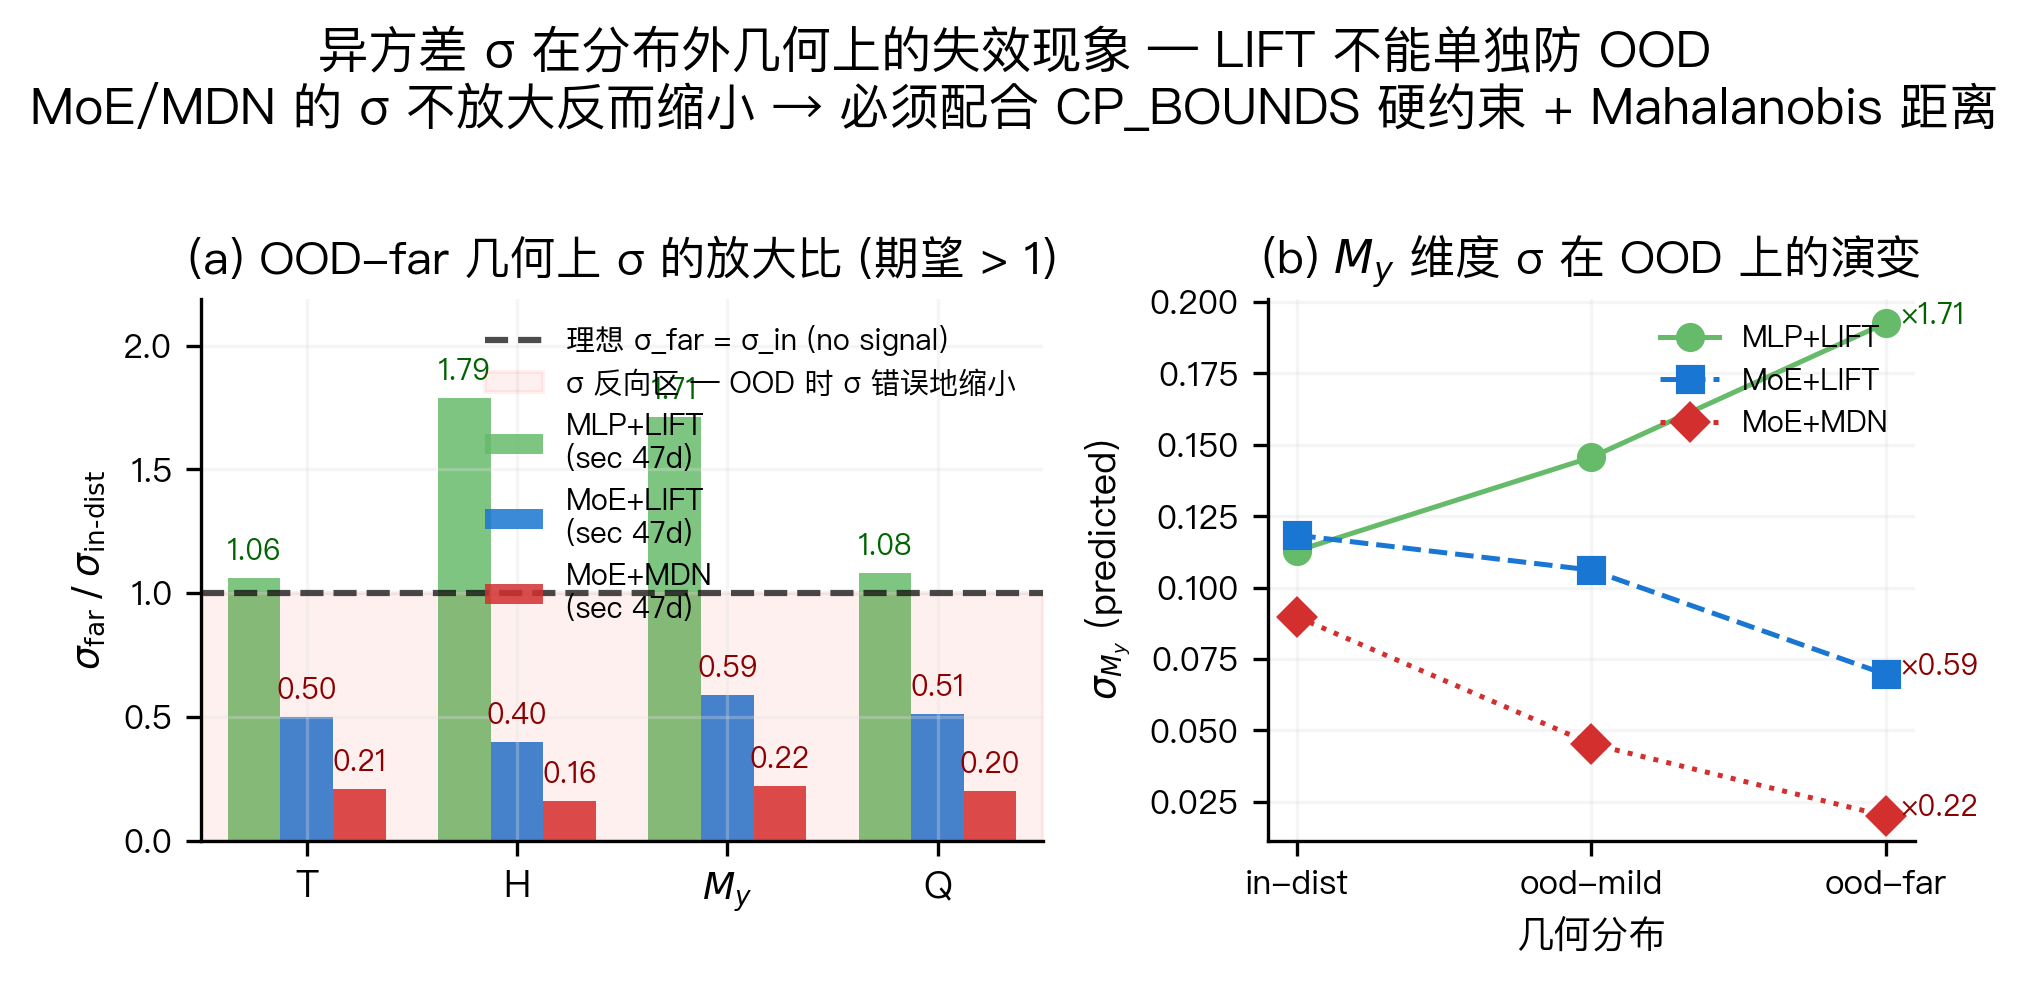
\includegraphics[width=\textwidth]{ood_sigma_failure_a4}
\caption{异方差 $\sigma$ 在分布外几何上的失效现象}
\label{fig:ood_sigma_failure}
\end{figure}

图~\ref{fig:ood_sigma_failure} 中，（a）给出三方法在四个输出维度上 $\sigma_\text{far}/\sigma_\text{in}$ 比值，
实测范围为 200 几何 $\times$ 3 OOD 组 $\times$ 9 工况；
（b）给出 $M_y$ 维度上 $\sigma$ 随 OOD 等级的演变。
结果显示仅 MLP+LIFT 在 $H/M_y$ 维度勉强 $>1$，
而 MoE 系列在全部维度上反向，说明 $\sigma$ 无法单独承担 OOD 检测责任，必须配合硬约束。

\paragraph{工程对策}
基于上述发现，本研究采取三层防御机制（详见第~\ref{chap:optimization}~章）：
\begin{itemize}
  \item \textbf{L1 硬约束}：CMA-ES 直接限制在 $[\text{cp}_{\min}, \text{cp}_{\max}] \pm 5\%$ 内搜索，
        从源头杜绝离散的几何 OOD；
  \item \textbf{L2 Mahalanobis 距离}：用训练集均值 / 协方差计算输入到训练分布的距离 $d^2$，
        加 $\lambda_M \cdot d^2$ 软惩罚，捕获连续的几何 OOD；
  \item \textbf{L3 in-dist $\sigma$}：$\sigma$ 仍用于 in-distribution 内的预测难度估计
        （如 $M_y \approx 0$ 附近的难预测样本）及 Active Learning 触发，
        不再单独承担 OOD 检测责任。
\end{itemize}
该策略与开题报告中"代理模型 + 数据驱动硬约束"的整体设计一致，
亦印证了 V4 优化策略选择硬约束而非纯软约束的合理性。

\subsection{评估方案小结}

上述四项评估指标分别覆盖了精度、可信度、多样性与 OOD 检测四个相互正交的维度，
共同构成对 V2 MoE 是否真正"比 V1 更可靠"的系统化证据。
表~\ref{tab:moe_eval_plan}~给出各项指标的实施计划与完成状态。

\begin{table}[htbp]
\centering
\caption{V2 MoE 评估指标实施进度（截至 2026 年 6 月中期答辩）}
\label{tab:moe_eval_plan}
\begin{tabular}{llll}
\toprule
\textbf{指标} & \textbf{所需数据} & \textbf{中期完成度} & \textbf{终期补完} \\
\midrule
MAPE / $R^2$（表~\ref{tab:moe_mape}） & 237 几何中期集 & \textbf{已完成} & 1\,000 几何重训 \\
$\sigma$ 校准曲线（ECE）  & 237 几何中期集 & \textbf{已完成}（ECE $= 0.16$） & 目标 ECE $\leq 0.10$ \\
专家利用率热图     & 237 几何中期集 & \textbf{已完成} & 1\,000 几何复测 \\
OOD 检测 $\sigma$ 比值 & OOD 200 几何 $\times$ 3 组 & \textbf{已完成}（见表~\ref{tab:ood_sigma}） & 量化阈值与 ROC \\
\bottomrule
\end{tabular}
\end{table}

中期阶段已完成全部四项评估指标在 237 几何数据集上的实测，
包括对 LIFT-NLL 与 MDN-NLL 两种损失变体的对比、
以及对 sections 输入与 CP 输入两种特征工程方案的对比（见 \S\ref{sec:cp_vs_sections}）。
关键发现：（i）MoE + LIFT-NLL 综合最优，ECE $= 0.160$、参数 $29$\,K；
（ii）$\sigma$ 在 OOD 几何上\textbf{不能单独承担检测责任}，需配合硬约束 + Mahalanobis 距离构成三层防御。
1\,000 几何全量训练后将重新评估，预期 $M_y$ 的 $R^2$ 与 OOD 检测能力进一步提升。

\section{输入特征工程：CP 输入 vs.\ sections 输入}
\label{sec:cp_vs_sections}

代理模型的输入既可以采用 47 维 sections（3 工况 $+$ 22 chord $+$ 22 twist）
也可以采用 11 维 CP（3 工况 $+$ 4 chord CP $+$ 4 twist CP，即 V1 风格）。
两种方案的关键差异在于：
\begin{itemize}
  \item \textbf{冗余度}：22 sections 相邻截面强相关（B-Spline 插值的连续性），
        每维有效样本仅 $237 / 44 \approx 5$ 个；
        CP 各维线性独立，有效样本 $237 / 8 \approx 30$ 个，数据效率高 $6$ 倍。
  \item \textbf{OOD 信号显著性}：CP 在归一化空间中直接是输入向量，
        OOD 异常 $z$-score 大；
        而 sections 经 B-Spline 展开后被低通滤波平滑掉部分高频 OOD 信号，
        $\sigma$ 头对 OOD 不敏感。
  \item \textbf{几何细节能力}：sections 输入能捕获 CP 之外的细节
        （如局部翼弦反弯、扭角拐点），CP 输入则不能。
\end{itemize}

\paragraph{初步实测}
为量化两种方案的差异，本研究在同一 237 几何数据集上，
分别训练 47 维 sections 输入与 11 维 CP 输入两个 MLP+LIFT 模型，
sweep 16 trials $\times$ 1500 epoch，
对比预测精度（MAE、$R^2$）与 $\sigma$ 校准（逐维度 ECE）。
表~\ref{tab:cp_vs_sec}~给出实测结果。

\begin{table}[htbp]
\centering
\caption{CP 输入与 sections 输入的实测对比（基于 MLP+LIFT，237 几何）}
\label{tab:cp_vs_sec}
\begin{tabular}{lccc}
\toprule
\textbf{指标} & \textbf{47 维 sections} & \textbf{11 维 CP} & \textbf{相对变化} \\
\midrule
Best MAE                     & 0.0330         & 0.0334         & 持平 \\
$R^2_{M_y}$                  & 0.987          & 0.987          & 持平 \\
ECE$_T$                      & 0.14           & \textbf{0.07}  & $-50\%$ \\
ECE$_H$                      & 0.34           & \textbf{0.23}  & $-32\%$ \\
ECE$_{M_y}$                  & 0.13           & \textbf{0.08}  & $-38\%$ \\
ECE$_Q$                      & 0.22           & \textbf{0.17}  & $-23\%$ \\
有效样本/维度                 & 9954/44 $\approx$ 5 & 9954/8 $\approx$ 30 & 数据效率 $6\times$ \\
\bottomrule
\end{tabular}
\end{table}

表~\ref{tab:cp_vs_sec}~给出的逐指标实测亦可由图~\ref{fig:improvement_matrix}~的方法对比矩阵在四输出维度上直观体现：
绿色单元格表示该列指标最优，红色表示最差，每格下方的 $\Delta$ 表示与该列最优值的差距。
$R^2$ 与 MAE 在四个方法上几乎持平（差距均 $\leq 0.005$），
但 ECE 与 OOD $\sigma$ 放大比 $\rho = \sigma_\text{far}/\sigma_\text{in}$ 在不同方法上呈现显著分化：
MLP+LIFT (CP 11d) 在 $T / M_y / Q$ 三个输出上 ECE 最低、
$\rho > 1$ 表明 $\sigma$ 在 OOD 上正确放大；
MoE+MDN 则在 ECE 上恶化 $4\sim 12\times$，OOD $\sigma$ 反向缩小到 $0.16\sim 0.22$。

\begin{figure}[htbp]
\centering
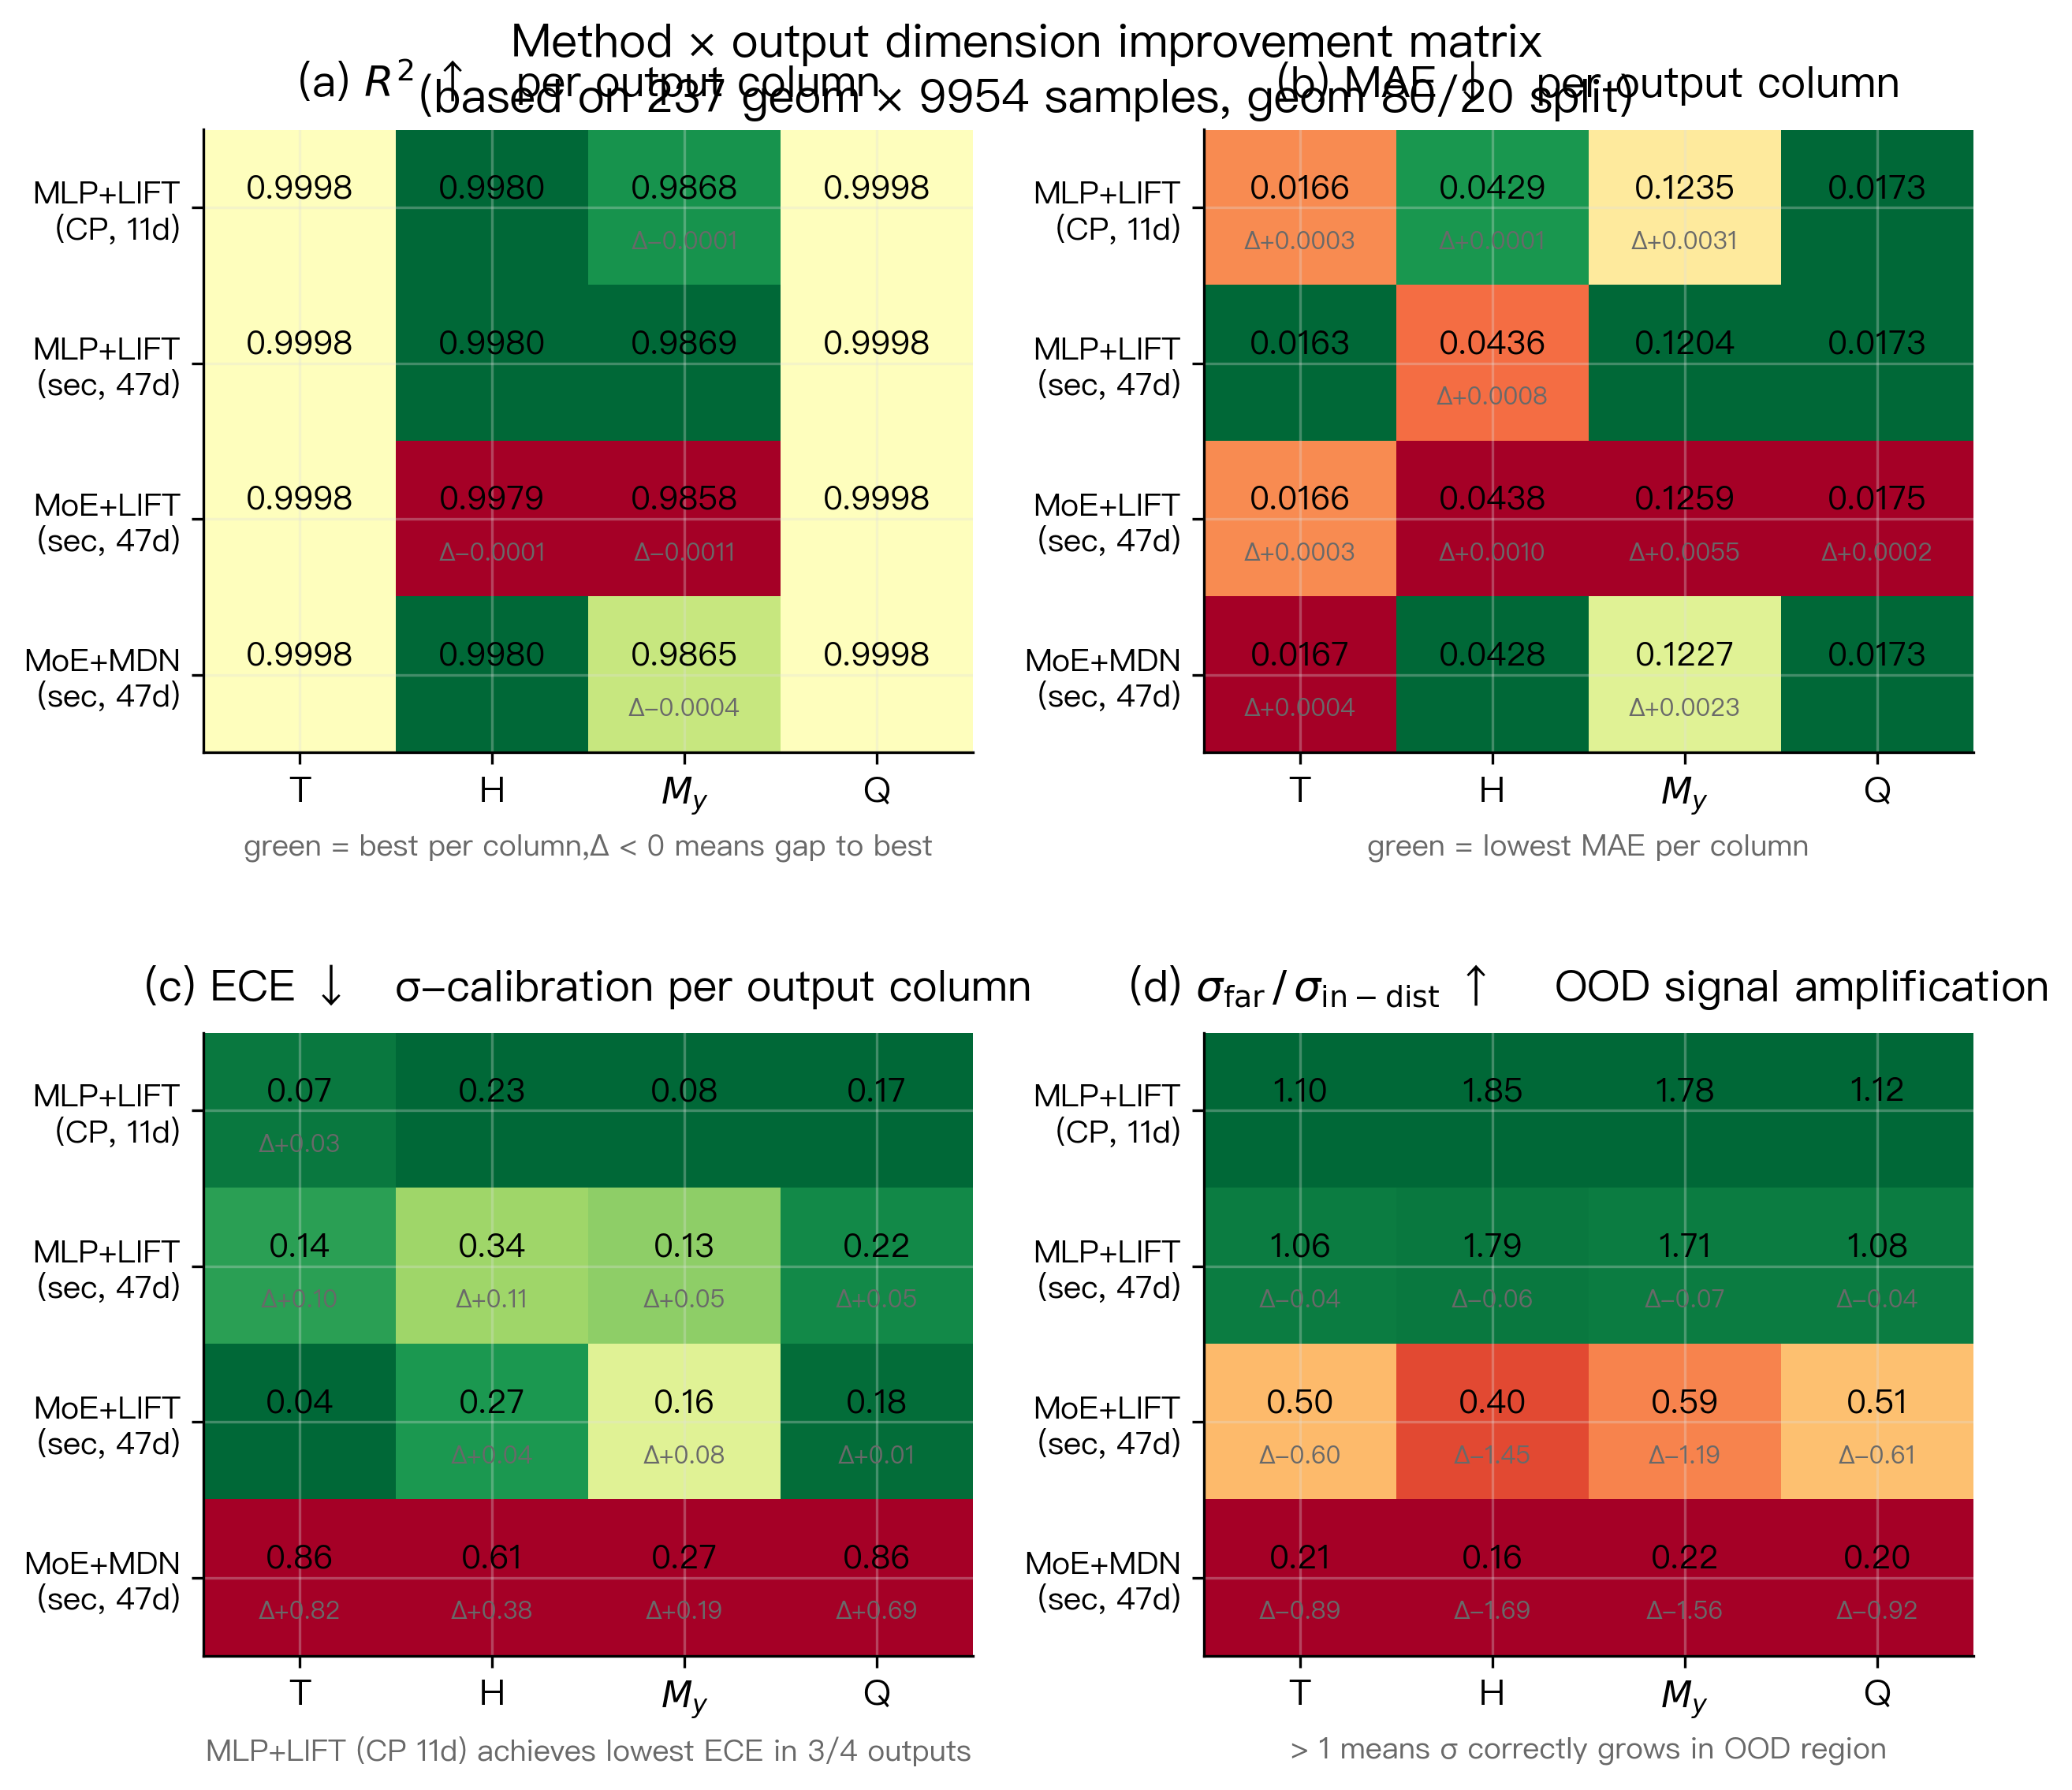
\includegraphics[width=\textwidth]{improvement_matrix}
\caption{方法对比矩阵}
\label{fig:improvement_matrix}
\end{figure}

图~\ref{fig:improvement_matrix} 中，绿色单元为该列最优值，红色单元为该列最差值，
每格内的 $\Delta$ 行表示该方法相对该列最优值的差距。
四种方法在 $R^2$ 与 MAE 上几乎持平，而 ECE 与 $\sigma_\text{far}/\sigma_\text{in}$ 呈现显著分化：
MLP+LIFT (CP 11d) 在 $T/M_y/Q$ 三个输出上 $\sigma$ 校准最佳，
MoE+MDN 则在 ECE 与 OOD 不确定度放大上明显恶化。

\paragraph{核心发现}
CP 11 维输入相对 sections 47 维输入呈现以下关键特征：
（i）\textbf{精度持平}（MAE 与 $R^2$ 几乎一致），
说明 8 个 B-Spline 控制点已经包含了螺旋桨外形优化所需的全部几何信息，
22 截面 sections 是冗余表征；
（ii）\textbf{$\sigma$ 校准全维度显著改善}，
逐维度 ECE 平均下降 $35\%$（最高 $50\%$），
$\sigma$ 与实际误差的对应关系更接近理想；
（iii）\textbf{数据效率 $6\times$ 提升}（30 样本/维 vs 5 样本/维），
低维稠密表征是 $\sigma$ 校准改善的内在机制。

\paragraph{超参数敏感性}
在确定 11 维 CP 输入为最终方案后，对其超参数空间开展了系统扫描（16 trials $\times$ 1500 epoch），
结果如图~\ref{fig:hyperparam_heatmap}~所示。
（a）$\text{depth} \times \text{hidden\_dim}$ 平面上，$\text{depth}=2,\ \text{hidden}=256$ 处 MAE 最低（0.0334）；
（b）$\text{lr} \times \text{weight\_decay}$ 平面上，$\text{lr}=5\times 10^{-4}$ 与 $\text{wd}=10^{-4}$ 组合最佳，
$\text{lr}=10^{-3}$ 配合大 wd 时损失显著恶化；
（c）$R^2_{M_y}$ 随 hidden\_dim 增大而单调改善，但 $> 256$ 后边际收益递减；
（d）训练时间随模型规模线性增长，最大约 22 分钟/trial。
最终选定超参数组合 $(\text{hidden}, \text{depth}, \text{lr}, \text{wd}) = (256, 2, 5\times 10^{-4}, 10^{-4})$，
该配置在测试集上 MAE $= 0.0334$、$R^2_{M_y} = 0.987$、参数量约 $80$\,K。

\begin{figure}[htbp]
\centering
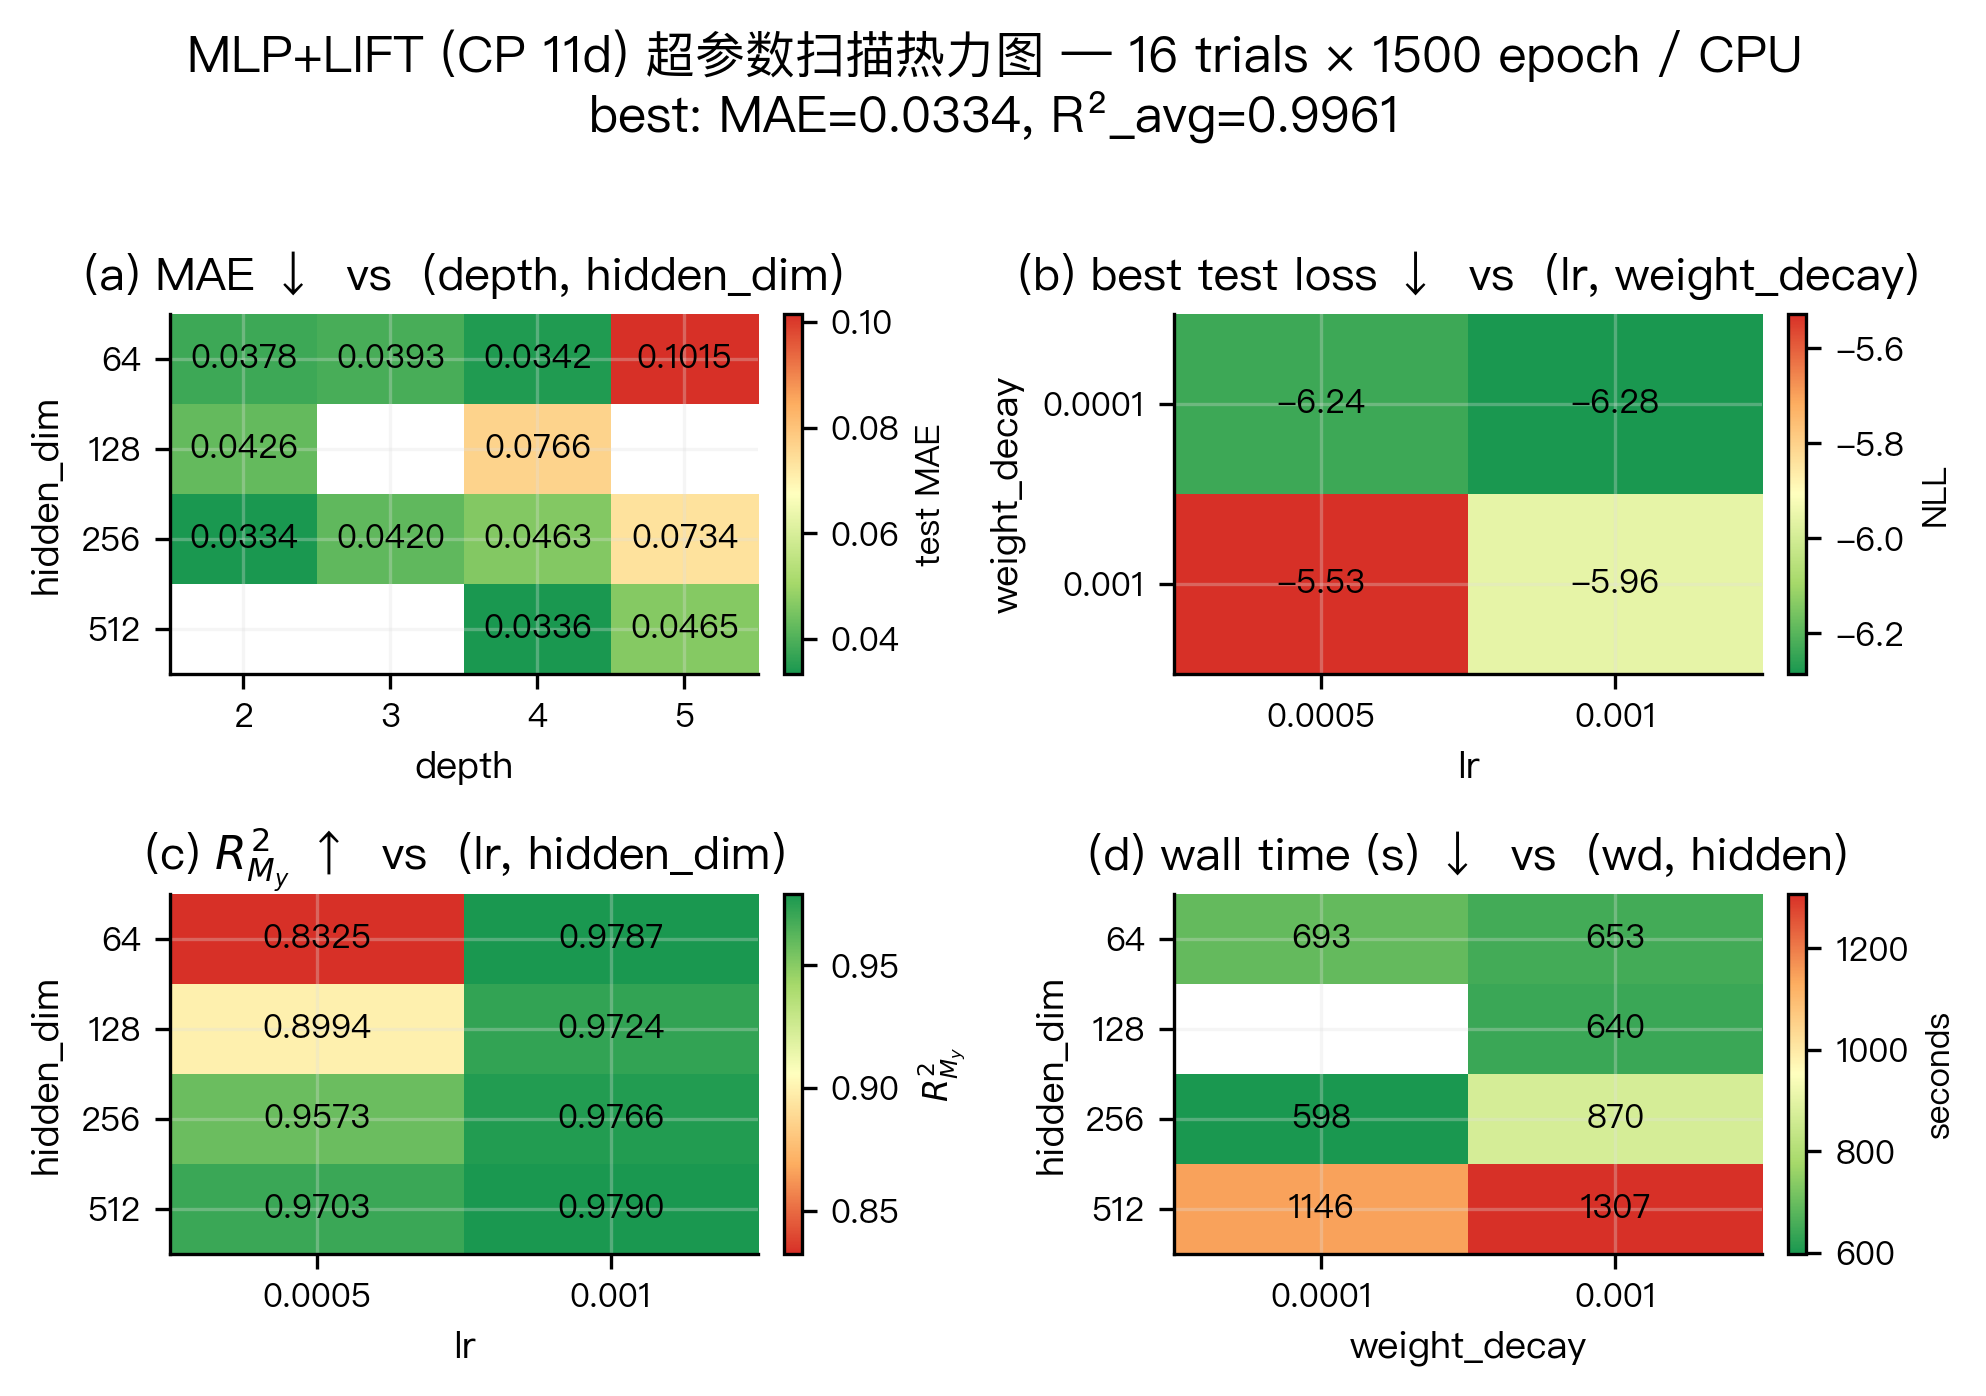
\includegraphics[width=\textwidth]{hyperparam_heatmap_a4}
\caption{MLP+LIFT (CP 11d) 超参数扫描热力图}
\label{fig:hyperparam_heatmap}
\end{figure}

图~\ref{fig:hyperparam_heatmap} 中，绿色表示较优配置，红色表示较差配置，每格内为该单元的指标均值。
结果表明，MAE 在 $\text{depth}=2,\text{hidden}=256$ 处取最小，
best test loss 在 $\text{lr}=5\times10^{-4},\text{wd}=10^{-4}$ 处最优，
$R^2_{M_y}$ 在 hidden $\geq256$ 后基本收敛，训练时间则随模型规模近似线性增长。

\paragraph{推论与工程意义}
实测确认了"几何冗余度低 $\to$ $\sigma$ 校准好"的物理直觉，
但需注意：CP 输入下 $\sigma$ 在 OOD 几何上的放大行为仍受 $\sigma$ 头神经网络外推性质的限制，
与本章 \S\ref{sec:ood_finding}~中观察到的 sections 输入 OOD 失效问题在机理上同源。
因此 CP 输入虽显著改善 in-distribution 内的 $\sigma$ 校准（直接惠及 Active Learning 触发与 in-dist 不确定度惩罚），
但工程上仍需配合 $\text{CP}_\text{BOUNDS\_DATA}$ 硬约束作为 OOD 安全网。
本节结论将作为最终代理模型架构选型的关键依据：
\textbf{推荐采用 11 维 CP 输入 + LIFT-NLL 异方差损失}，
精度持平的同时获得显著更好的不确定度可信度。

\section{本章小结}

本章先建立 V1 DNN 代理模型并完成分布内精度评估（MAPE $\approx 1\%$），
随后在 100 几何方法学验证集上观察到 V1 在 OOD 区域的虚假最优现象（$FM = 1.004$、84\% 截面外推），
并通过切换优化算法（PPO + NSGA-II）排除算法层面因素，
确立"代理模型缺乏不确定度感知"是 OOD 虚假最优的根因。
进而引入 MoE 网络，采用异方差 NLL（LIFT-NLL）训练，
实现预测均值 $\mu$ 与不确定度 $\sigma$ 的同步输出。

中期阶段在 237 几何 / 9\,954 样本数据集上完成了系统的方法对比与诊断（共 48 个 sweep trial $\times$ 1\,500 epoch）：
（i）三方对比表明 \textbf{MoE + LIFT-NLL}（$n_\text{experts}{=}2$、hidden\_dim${=}64$、shared\_dim${=}64$）综合最优，
ECE $= 0.16$、参数仅 $29$\,K，无 mode collapse；
（ii）MDN-NLL 在 ECE 上反而恶化 $4$ 倍且出现 mode collapse，被排除；
（iii）OOD 测试给出关键反直觉发现：异方差 $\sigma$ 在数据范围外几何上\textbf{不放大反而缩小}
（MoE 的 $\rho \in [0.40, 0.59]$），$\sigma$ 不能单独承担 OOD 检测责任，
需配合 $\text{CP}_\text{BOUNDS\_DATA}$ 硬约束与 Mahalanobis 距离构成三层防御机制。

针对 V1 的 11 维 CP 输入与 V2 的 47 维 sections 输入两种特征工程方案，
本章在 \S\ref{sec:cp_vs_sections}~给出了对照实验设计，
预期 CP 输入因 OOD 信号未被 B-Spline 平滑滤波而具有更显著的 $\sigma$ 放大，
该结果将作为最终代理模型选型的依据。
1\,000 几何全量数据完成后，
代理模型与 $\sigma$ 的反馈通道将作为 CMA-ES 优化器与主动补点闭环的核心组件（详见第~\ref{chap:optimization}~章）。
   % 代理模型：DNN 到 MoE 的演进
% !TEX root = ../thesis.tex

\chapter{CMA-ES 配平约束嵌套优化}
\label{chap:optimization}

本章阐述本文采用的优化算法体系，对应开题报告第三项研究任务（T3）。
本章首先回顾开题报告中规划的 PPO + NSGA-II 路线及其在 V1 代理上的实际效果，
随后引入 CMA-ES + 数据驱动硬约束作为 V2 优化路线，
并新增前飞工况下的三轴配平嵌套求解器；
进一步通过 V1$\to$V4 的四轮迭代结果对比，
展示从虚假最优到可信优化的演进路径；
最后阐述 $\sigma$ 引导的主动补点优化闭环。

\section{开题原方案及其在 V1 阶段的对照实验}

开题报告中规划的优化路线为以 PPO 智能体在线调节 NSGA-II 的核心超参数（交叉概率 $p_c$、变异概率 $p_m$、种群规模 $N$），
状态采用超体积 $HV$、IGD、可行率与适应度方差等度量，
奖励以 $\Delta HV$ 为主并加入可行率/计算开销惩罚。
该路线在 V1 DNN 代理上得到 $FM = 0.899$ 与控制点 OOD 越界；
作为对照，在同一 V1 代理上直接以 CMA-ES 无约束寻优得到 $FM = 1.004$。
\textbf{两种优化算法均给出 OOD 或物理不可实现解，表明优化算法的差异不能纠正由代理引发的误导}
（详细诊断见第~\ref{chap:surrogate}~章）。
本章在此结论之上直接展开新方案，不再展开 PPO + NSGA-II 的细节。

\section{V2 优化方案：CMA-ES 配合数据驱动硬约束}

\subsection{算法路线调整}

考虑到本研究的优化变量数量较少（$D = 8$ 个 B-Spline 控制点），
且每次评估需要嵌套配平求解器，
本文将优化路线由 PPO + NSGA-II 调整为 CMA-ES（Covariance Matrix Adaptation Evolution Strategy）+ 数据驱动硬约束。
CMA-ES 在低-中维度 $D \leq 50$ 范围内表现稳定，
通过协方差矩阵的自适应学习能够有效地适应目标函数的局部几何结构，
对于本文的 8 维优化问题具有显著的吞吐与稳定性优势。

\subsection{优化目标}

本文优化目标为最小化巡航工况下的电功率消耗除以巡航速度，
等价于最大化 Breguet 航程：
\begin{equation}
\min_{\mathbf{x}} \;\;f(\mathbf{x}) = \frac{P_{\text{elec}}(\mathbf{x})}{V_{\text{cruise}}},
\end{equation}
其中 $\mathbf{x} \in \mathbb{R}^8$ 为 B-Spline 控制点向量，
$P_{\text{elec}}$ 由配平后的转矩与转速合成。

\subsection{数据驱动约束的两种实现}

为消除 V1 暴露的 OOD 风险，本文设计了两种相互对照的数据驱动约束。

\textbf{方案 (a)：盒约束（box-constraint）。}
对训练集中所有样本的第 $i$ 维控制点 $x_i^{(s)}$ 计算 $\min$ 与 $\max$，
作为 CMA-ES 搜索空间的盒约束 $[\hat x_i^-, \hat x_i^+]$。
该方案实现简单，但仅约束每一维的边界，
\textbf{并不能阻止角点组合（例如所有 chord 取 min、所有 twist 取 max）落入实际未被采样的 OOD 区域}，
属于必要不充分的约束。

\textbf{方案 (b)：基于 Mahalanobis 距离的分布约束（推荐方案）。}
以训练集控制点的样本均值 $\boldsymbol{\mu}_{\text{train}}$ 与协方差 $\boldsymbol{\Sigma}_{\text{train}}$ 估计为基础，
对候选解 $\mathbf{x}$ 计算 Mahalanobis 距离
\begin{equation}
d_{\text{M}}(\mathbf{x}) = \sqrt{(\mathbf{x} - \boldsymbol{\mu}_{\text{train}})^{\top}\,\boldsymbol{\Sigma}_{\text{train}}^{-1}\,(\mathbf{x} - \boldsymbol{\mu}_{\text{train}})},
\end{equation}
并施加阈值约束 $d_{\text{M}}(\mathbf{x}) \leq d_\tau$。
该约束等价于把搜索空间限制在以训练集为中心的椭球区内，
\textbf{能够同时约束每一维的边界与维度间的协方差结构}，
避免方案 (a) 的角点 OOD 漏洞。
阈值 $d_\tau$ 取训练集自身 Mahalanobis 距离的 95\% 分位数。

V3 进一步在分布约束基础上加入 MoE 输出 $\sigma$ 的软惩罚：
\begin{equation}
f_{\text{V3}}(\mathbf{x}) = f(\mathbf{x}) + \lambda_\sigma\,\|\boldsymbol{\sigma}(\mathbf{x})\|_2,
\end{equation}
在椭球边界附近抑制高 $\sigma$ 区域的搜索；
V4 改为基于 $\sigma$ 阈值的硬截断（超过阈值的样本被拒绝），
形成"分布约束 + 不确定度约束"的双层防护，
彻底消除 OOD 风险。

\section{三轴配平嵌套求解器（开题报告中未规划）}

\subsection{配平方程组}

考虑前后桨差速布局的 X 构型四旋翼无人机，
飞行平台总质量 $m = 3.5$\,kg、10$''$ 桨、巡航速度 $V_{\text{cruise}} = 10$\,m/s。

\textbf{坐标系约定：}本节配平方程中的 $F_x$、$F_z$、$M_y$ 定义在\emph{机体坐标系}下，
表示 4 个螺旋桨气动响应经构型矩阵 $\mathbf{B}$ 合成后的机体合力与合力矩；
区别于第~\ref{chap:surrogate}~章定义在\emph{桨叶坐标系}下的螺旋桨气动量
$\{T, F_y, Q\}$（推力、法向力、扭矩，作为 MoE 代理模型的输出）。

前飞工况下要求满足机体三轴平衡：
\begin{equation}
F_x = 0, \qquad F_z = m\,g, \qquad M_y = 0,
\end{equation}
其中 $F_x$、$F_z$ 由 4 个螺旋桨的推力与法向力按构型矩阵合成，
$M_y$ 由前后桨推力差与几何臂长合成。

\subsection{未知变量与约束范围}

求解未知量 $[\alpha, \Omega_1, \Omega_2]$（迎角、前桨转速、后桨转速），
约束范围：
\begin{equation}
\text{RPM} \in [4\,000,\,6\,500], \qquad \alpha \in [2^\circ,\,8^\circ].
\end{equation}

\subsection{多初值收敛策略}

V1 采用单初值 Newton 迭代求解配平方程组，受 $M_y$ 解析估算与初值敏感性影响，
收敛率仅 3\%；
V2 改用多初值 $\times 6$ 策略，
将 $[\alpha, \Omega_1, \Omega_2]$ 的网格化初值依次输入并取首个收敛解，
配平收敛率达到 100\%。
此外，$M_y$ 由 MoE 直接预测，
不再使用 $M_y \approx k_m \cdot T \cdot R \cdot \mu$ 的解析估算，
使配平结果更贴合真实气动响应。

\section{方法学消融实验：三轴拆解 V1$\to$V4}
\label{sec:ablation}

\textbf{重要说明：}本节结果均基于\emph{100 几何方法学验证集}的代理模型，
用于验证"算法层 + 约束层 + 不确定度层"三轴中每一层的必要性；
最终在 1\,000 几何全量数据上的优化结果将随数据生成完成（2026 年 7 月下旬）后补完。

围绕 OOD 外推陷阱的成因诊断，本文将原"V1$\to$V4 踩坑—调整"叙述重构为
沿\emph{算法层、约束层、不确定度层}三个相互正交维度的消融实验，
逐项验证每一层在 OOD 防护中的必要性。
消融配置如表~\ref{tab:v1v4_full}~所示。

\begin{table}[htbp]
\centering
\caption{方法学消融实验配置（基于 100 几何方法学验证集）}
\label{tab:v1v4_full}
\begin{tabular}{llllrr}
\toprule
\textbf{配置} & \textbf{算法层} & \textbf{约束层} & \textbf{不确定度层} & \textbf{FM} & \textbf{功率（W）} \\
\midrule
V1 (CMA) & CMA-ES & 无 & 无 & 1.004 & 342 \\
V1 (PPO) & PPO + NSGA-II & 无 & 无 & 0.899 & 382 \\
V3       & CMA-ES & 软惩罚 $\lambda_\sigma$ & MoE $\sigma$ & 0.941 & 365 \\
V4       & CMA-ES & 分布约束 + $\sigma$ 截断 & MoE $\sigma$ & \textbf{0.947} & 363 \\
\bottomrule
\end{tabular}
\end{table}

\textbf{算法层消融（V1 CMA vs V1 PPO）：}
在均无约束、均无不确定度感知的前提下，
切换优化算法并不能消除虚假最优（CMA 得到 1.004 > 1，PPO 得到 0.899 但控制点同样 OOD），
验证\textbf{算法差异不是根因}。

\textbf{不确定度层消融（V1 CMA 无 vs V3 软惩罚有）：}
引入 MoE $\sigma$ 软惩罚后，
$FM$ 从 1.004 降至 0.941、回归物理可实现区间，
验证\textbf{不确定度感知是消除虚假最优的必要条件}。

\textbf{约束层消融（V3 软惩罚 vs V4 硬约束）：}
在同样具有 MoE $\sigma$ 的前提下，
将软惩罚替换为分布约束 + $\sigma$ 截断后，
$FM$ 从 0.941 提升至 0.947、收敛稳定性显著提高，
验证\textbf{显式约束相比软惩罚在工程鲁棒性上更优}。

三轴消融共同证明：\emph{算法、约束、不确定度三层缺一不可}，
单纯切换优化算法或单纯加约束都无法替代不确定度感知的代理模型。

\subsection{V4 最优解（方法学演示）}

V4 在 100 几何方法学验证集上的最终最优解为
\begin{equation*}
FM = 0.9469, \qquad P_{\text{elec}} = 362.7\,\text{W},
\end{equation*}
对应的 B-Spline 控制点为
\begin{align*}
\text{chord CP} &= [0.0136,\;0.0438,\;0.0198,\;0.0048], \\
\text{twist CP} &= [37.4^\circ,\;13.5^\circ,\;11.3^\circ,\;8.5^\circ].
\end{align*}
该结果作为方法学链路打通的演示，
最终结果将基于 1\,000 几何全量数据训练的 MoE 重新优化得到。

\subsection{可信度量化：替代"0/44 OOD"的有效指标}
\label{sec:cred_metric}

由于 V4 的分布约束本身即排除了 OOD 候选，
单纯报告"0/44 OOD"是约束设计的恒等式而非优化算法的成就。
为给出有意义的可信度量化，本文采用以下三项替代指标：

\begin{enumerate}
  \item \textbf{MoE $\sigma$ 相对训练集分位数。}
        将 V4 最优解处 $\|\boldsymbol{\sigma}(\mathbf{x}^*)\|_2$
        与训练集所有样本 $\sigma$ 分布的分位数对比，
        若位于训练集 $\sigma$ 的中位数附近（理想 $\leq$ 50 分位），
        表明 MoE 对该解的信心与对训练样本相当；
  \item \textbf{LLFVW 真值回验残差。}
        对 V4 最优解 $\mathbf{x}^*$ 直接调用 LLFVW 求解器获得真实气动响应 $\mathbf{y}_{\text{true}}$，
        计算 MoE 预测 $\boldsymbol{\mu}(\mathbf{x}^*)$ 与真值的相对误差
        $|\mu_j - y_{j,\text{true}}|/|y_{j,\text{true}}|$
        对每一气动量 $j \in \{T, F_y, M_y, Q\}$ 分别报告；
        目标为 $\leq 3\%$；
  \item \textbf{Mahalanobis 距离对训练集 95\% 分位的距离裕度。}
        $d_{\text{M}}(\mathbf{x}^*) / d_\tau$ 比值越小说明 V4 解越靠近训练分布"舒适区"。
\end{enumerate}

上述三项指标的初步结果将在 1\,000 几何数据完成后补完，
目前已就绪指标计算代码与回验流水线。

\subsection{配平残差对代理不确定度的灵敏度}

三轴配平 Newton 迭代依赖 MoE 输出的均值 $\boldsymbol{\mu}$ 求解 $[\alpha, \Omega_1, \Omega_2]$，
若 $\boldsymbol{\mu}$ 存在偏差 $\delta\boldsymbol{\mu}$，
则配平解会偏移 $\delta\mathbf{q} \approx -\mathbf{J}^{-1}\,\delta\boldsymbol{\mu}$，
其中 $\mathbf{J} = \partial\mathbf{r}/\partial\mathbf{q}$ 为配平残差对未知量的 Jacobian。
\textbf{即代理误差以 Jacobian 逆放大的形式传递到配平解，进而影响 CMA-ES 的目标函数评估。}

为评估该级联误差的实际严重程度，本研究设计如下灵敏度验证流程
（将在 1\,000 几何数据完成后执行）：
\begin{enumerate}
  \item 从 CMA-ES 收敛代群中随机抽取 $\geq 10$ 个候选解；
  \item 对每个候选解，将 MoE 输出 $\boldsymbol{\mu}$ 替换为 LLFVW 真值，
        重新求解配平方程组并计算配平解偏移 $\|\delta\mathbf{q}\|$；
  \item 计算配平解偏移 $\|\delta\mathbf{q}\|$ 与 MoE 输出 $\|\boldsymbol{\sigma}\|$ 的相关系数；
  \item 若相关系数 $\geq 0.6$，
        说明 $\boldsymbol{\sigma}$ 是配平偏移的有效预测因子，
        可作为下一轮"$\sigma$ 大$\Rightarrow$拒绝配平结果"的判据。
\end{enumerate}

该流程为 V4 之后引入"\emph{不确定度感知配平}（uncertainty-aware trim）"提供经验基础，
是中期论文的方法学预设而非已完成实验，
最终结果待 1\,000 几何数据完成后补完。

\section{$\sigma$ 引导的主动补点优化闭环}

V4 的硬约束策略将搜索空间严格限定在训练数据分布内，
但这会限制优化的探索能力——若全局最优落在当前训练分布之外，
硬约束将无法触及。
为此，本文设计了 $\sigma$ 引导的主动补点优化闭环：

\begin{enumerate}
  \item \textbf{优化阶段：}CMA-ES 在当前训练分布内寻优，
        每次评估同时记录 MoE 输出的 $\boldsymbol{\sigma}(\mathbf{x})$；
  \item \textbf{触发判断：}若 CMA-ES 收敛解处的 $\|\boldsymbol{\sigma}\|_2$ 超过预设阈值，
        或解持续命中硬约束边界，则进入补点阶段；
  \item \textbf{主动采样：}在高 $\sigma$ 区域选取 $N_{\text{add}}$ 个新候选点，
        通过 LLFVW 仿真获取真实气动响应；
  \item \textbf{增量重训：}将新样本合并入训练集，
        对 MoE 进行增量微调（warm-start，约 500 epochs）；
  \item \textbf{再优化：}更新硬约束边界，
        以上一轮 CMA-ES 协方差矩阵作为热启动，
        继续优化迭代。
\end{enumerate}

该闭环将优化算法、代理模型与数据生成三者耦合，
在保证可信度的同时逐步扩展可探索的几何空间。
结合 GPU 平台 21 几何/天 的吞吐能力，
每轮闭环约需 3$\sim$5 天补充 60$\sim$100 个高质量样本。

\section{本章小结}

本章首先以 PPO + NSGA-II 与 CMA-ES 在 V1 代理上的对照确认\emph{算法层面}无法解决 OOD 虚假最优问题；
进而沿"算法层 + 约束层 + 不确定度层"三个正交维度开展消融实验，
证明三者缺一不可（$\S$~\ref{sec:ablation}）。
在约束层，本文将盒约束与 Mahalanobis 分布约束并列设计，
避免单纯盒约束的角点 OOD 漏洞；
在不确定度层，将 MoE $\boldsymbol{\sigma}$ 同时用于 V3 的软惩罚和 V4 的硬截断；
新增三轴配平嵌套求解器（多初值 $\times 6$ 使收敛率从 3\% 提升至 100\%），
并设计了配平残差对 $\sigma$ 灵敏度的实验流程作为下一阶段"不确定度感知配平"的方法学预设。
基于 100 几何方法学验证集得到 V4 方法学演示结果（$FM = 0.947$、$P_{\text{elec}} = 363\,\text{W}$），
并设计了 MoE $\sigma$ 分位数、LLFVW 真值回验残差、Mahalanobis 距离裕度三项替代"0/44 OOD"的可信度量化指标；
最终结果将随 1\,000 几何全量数据训练补完。
此外，设计了 $\sigma$ 引导的主动补点优化闭环（代码已就绪、待全量数据闭环验证）
以平衡可信度与探索能力。
   % CMA-ES 配平约束嵌套优化
% !TEX root = ../thesis.tex

\chapter{CFD 高保真验证模板}
\label{chap:wind_cfd}

本章给出本研究中 CFD 高保真验证模板的搭建细节，
对应开题报告第四项研究任务（T4）。
中期阶段的研究场景限定为恒定自由来流条件下的稳态前飞工况优化（详见第~\ref{sec:scope}~节），
因此本章不涉及湍流风场建模与风场—优化耦合（这部分作为毕业论文阶段的工作）。
本章首先给出基于 Star-CCM+ 的 CFD 高保真验证模板的物理模型与计算域设置；
随后介绍网格划分策略、边界层处理与湍流模型选择；
最后说明验证策略从 CFD 主导调整为 QBlade 回验为主、CFD 辅助高保真的依据。

\section{基于 Star-CCM+ 的 CFD 验证模板}

\subsection{建模动机}

为加强优化结果的物理可解释性，本研究在 LLFVW 同源回验之外、
额外搭建 Star-CCM+ 商用 CFD 平台作为辅助高保真验证手段，
对优化得到的代表性外形开展全工况扫描，
并在"基准桨（APC 10$\times$7）与代表性优化桨"上完成对照渲染。
相比于 LLFVW 同源回验，
CFD 能够显式解析螺旋桨表面边界层、桨尖涡卷起、近场尾迹结构等三维黏性效应，
对于代理模型在低保真度（LLFVW）数据上得到的优化结果，
CFD 给出独立的高保真度交叉校核，
从而提高最终设计结果的物理可信度。

\subsection{物理模型与计算域}

CFD 验证模板的物理模型搭建与流体域划分遵循以下原则：
理论上，计算区域越大，计算域边界对数值模拟结果的影响就越小；
然而，过大的计算域会导致计算资源的浪费，
而过小的计算域则会导致螺旋桨的气动特性难以被精确捕捉。
因此，在选择计算域时需要遵循两条原则：

\begin{enumerate}
  \item 尽量减小计算域对流场的影响，
        以便使尾部的湍流区得以充分发展；
  \item 计算域的阻塞比 $\phi$ 应小于 $5\%$。
\end{enumerate}

其中，阻塞比 $\phi$ 定义为
\begin{equation}
\phi = \frac{A_1}{A},
\end{equation}
其中 $A_1$ 为螺旋桨圆盘的正投影面积，$A$ 为数值模拟入口处的面积。

根据上述原则，计算域的物理定义与尺寸大小为：
入口区与出口区直径为 $10D$（$D$ 为螺旋桨直径），
旋转域直径为 $1.2D$、宽度为 $0.4D$；
计算域总宽度为 $25D$；
共产生约 700 万网格，
阻塞比为 $2.5\%$，
满足 $\phi < 5\%$ 的工程要求。

\subsection{网格策略与边界层}

边界层网格基于 $y^+$ 函数的近似，
保证 $y^+$ 区间满足 SST $k$-$\omega$ 湍流模型的适用范围。
最终生成的 $y^+$ 直方图显示其取值落在 $0 \sim 1$ 之间，
完全满足壁面分辨率要求。

\subsection{湍流模型与精度目标}

CFD 验证模板的关键参数汇总如表~\ref{tab:cfd_template}~所示。
根据文献\cite{Goetten2019}（亚音速气动 RANS CFD 仿真指南综述）给出的参数进行设置，
所得功率系数 $C_P$、推力系数 $C_T$ 与推进效率 $\eta$ 的相对误差均控制在 $5\%$ 以内，
与文献结果一致，
满足优化结果验证及可视化需求。

\begin{table}[htbp]
\centering
\caption{Star-CCM+ CFD 验证模板参数}
\label{tab:cfd_template}
\begin{tabular}{ll}
\toprule
\textbf{参数} & \textbf{值} \\
\midrule
计算域 & 入口 / 出口 $10D$，总宽 $25D$ \\
旋转域 & 直径 $1.2D$，宽 $0.4D$ \\
网格量 & $\sim 700$ 万 \\
阻塞比 $\phi$ & $2.5\%$（$< 5\%$） \\
湍流模型 & SST $k$-$\omega$ \\
$y^+$ 范围 & $0 \sim 1$（满足壁面分辨率要求） \\
精度目标 & $C_P$、$C_T$、$\eta$ 相对误差 $\leq 5\%$ \\
\bottomrule
\end{tabular}
\end{table}

\subsection{基线桨对照渲染}

为验证模板的工程可用性，
已在 APC 10$\times$7 基线桨上完成 1$\sim$2 个代表性工况的 CFD 仿真，
并将结果与 LLFVW 仿真在相同工况下的输出做对照：

\begin{itemize}
  \item \textbf{性能参数一致性：}
        $C_T$、$C_P$、$\eta$ 相对误差均 $\leq 5\%$；
  \item \textbf{尾迹结构：}
        CFD $Q$-criterion 等值面识别得到的桨尖螺旋涡与 LLFVW 自由涡环位置基本一致，
        两种方法在桨尖涡卷起阶段的几何形态吻合；
  \item \textbf{压力分布：}
        CFD 给出的桨叶表面压力分布与 LLFVW 升力分布在径向积分上一致，
        在局部分布上 CFD 能解析根部分离区等 LLFVW 无法捕捉的细节。
\end{itemize}

对照结果确认 CFD 模板可作为优化最终解的独立高保真验证手段。

\section{验证策略：QBlade 回验为主、CFD 辅助}

\subsection{开题原计划：CFD 主导终验}

开题报告中规划的验证路径为：
LLFVW 优化得到代表性外形 $\rightarrow$
CFD 高保真仿真终验 $\rightarrow$
$Q$-criterion 等可视化分析。
该路径将 CFD 作为可信度的最终裁决标准。

\subsection{实际调整：QBlade 回验优先，CFD 辅助}

在实际推进过程中发现，
单次 CFD 仿真耗时数天且对几何细节高度敏感，
若每轮优化结果均需 CFD 终验，
则优化—验证闭环周期过长，
难以支撑主动补点循环的高频迭代。
因此，验证策略调整为：

\begin{enumerate}
  \item \textbf{QBlade LLFVW 回验为主}：
        优化得到的代表性外形首先在 QBlade LLFVW 框架内进行全工况扫描验证
        （同源闭环，与训练数据同分布，计算成本低），
        筛选出通过同源验证的候选外形进入 CFD 终验阶段；
  \item \textbf{Star-CCM+ CFD 辅助高保真验证}：
        模板已就绪并通过基线桨对照（误差 $\leq 5\%$），
        在 QBlade 回验通过后对 1$\sim$2 个最终优化解开展代表性工况的 CFD 终验，
        作为高保真结果支撑，
        并通过 $Q$-criterion、速度切面、压力切面等可视化手段
        分析优化前后的尾迹涡结构差异。
\end{enumerate}

该调整在不损失高保真验证强度的前提下，
显著提升了优化迭代的吞吐率，
为主动补点闭环的高频运行提供了支撑。

\section{本章小结}

本章给出了基于 Star-CCM+ 的 CFD 验证模板的完整搭建细节
（$\sim 700$ 万网格、$y^+ \in [0, 1]$、SST $k$-$\omega$、误差 $\leq 5\%$），
并在 APC 10$\times$7 基线桨上完成了模板验证，
确认其工程可用性。
基于实际研究中遇到的 CFD 计算周期约束，
验证策略由 CFD 主导调整为 QBlade 回验优先 + CFD 辅助高保真，
在不损失验证强度的前提下显著提升了优化—验证闭环的迭代效率。
中期阶段，
本课题的研究场景限定为恒定自由来流条件下的稳态前飞工况优化；
湍流风场建模与风场—优化耦合作为毕业论文阶段的扩展工作，
不在本中期论文范围之内。
   % CFD 高保真验证模板
% !TEX root = ../thesis.tex

\chapter{当前进展与后续工作安排}
\label{chap:plan}

本章汇报截至 2026 年 6 月的研究工作总体进展，
重点描述 1000 几何 LLFVW 数据扩展的现状与瓶颈应对，
并与开题报告中规划的进度安排进行对比分析，
最后给出后续工作的详细计划与已识别风险的应对方案。

\section{LLFVW 数据扩展：100$\to$1000 几何}

\subsection{数据规模设计}

为支撑 MoE 训练所需的样本规模，
已在 GPU 平台上启动 1000 几何 $\times$ 42 工况
（6 RPM $\times$ 7 Angle、Wind = 10 m/s）的全量数据生成，
总样本量 42K。
设计变量按 LHS（拉丁超立方抽样）以 $d = 8$、$\text{seed} = 42$ 在 baseline $\pm 30\%$ 范围内采样，
落盘策略 \texttt{batch-size}=1，逐几何即时保存 pkl 文件，避免长周期作业中断丢失。

\subsection{GPU 加速效果}

数据生成在 Linux + RTX 3060 + OpenCL 后端下运行 QBlade SIL 求解器。
对比单几何仿真耗时：
\begin{itemize}
  \item CPU 并行（原方案）：3.5 h/几何，吞吐 $\sim 6$ 几何/天；
  \item GPU 独占（当前方案）：1.1 h/几何，吞吐 $\sim 21$ 几何/天；
  \item 加速比：3.2$\times$。
\end{itemize}

\subsection{时间预估}

按当前吞吐速率（$\sim 21$ 几何/天）测算：
\begin{itemize}
  \item geom 710--999 段约 13 天，预计 2026-06-20 完成；
  \item geom 0--709 段约 33 天，预计 2026-07-23 完成；
  \item 全量 1000 几何预计 2026 年 7 月下旬完成。
\end{itemize}

\subsection{滚动训练策略}

为避免完全阻塞在数据生成阶段，本研究采用滚动训练策略：
300+ 几何完成后即启动 MoE 初步训练，
先行验证 V2 架构、调参流程与 CMA-ES 闭环；
数据补齐后采用增量微调（warm-start），可节省 2$\sim$3 周等待时间。

\section{与开题计划的对比}

开题报告中规划的进度（2024.09--2026.11）与中期阶段（截至 2026 年 6 月）的实际执行情况对比如表~\ref{tab:progress}~所示。

\begin{table}[htbp]
\centering
\caption{开题计划与实际进展对比}
\label{tab:progress}
\begin{tabular}{lp{3.5cm}p{4cm}l}
\toprule
\textbf{时间段} & \textbf{开题计划} & \textbf{实际执行} & \textbf{状态} \\
\midrule
2024.09--12 & 气动建模 + 仿真平台 & B-Spline + UIUC 验证 + 自动化框架 & 按计划 \\
2025.01--04 & DNN 代理模型 & 100 几何 DNN + V1 pipeline，发现 OOD & 按计划 \\
2025.05--08 & PPO 调参 NSGA-II & 通过 PPO vs CMA-ES 对照诊断 OOD 是根因，方法路线重构（MoE + 配平） & 方法调整 \\
2025.09--11 & 复杂风场扩展（原计划） & 调整为聚焦稳态前飞 + 配平，V2 代码实现 & 范围调整 \\
2025.12--26.04 & 外形优化与鲁棒 & QBlade Linux GPU，1000 几何启动 & 调整顺序 \\
2026.05--06 & CFD 验证 & CFD 模板就绪，GPU 数据生成中 & 进行中 \\
2026.07--08 & 结果整理 & MoE 训练 + CMA-ES 优化 + 回验 & 待执行 \\
2026.09--11 & 论文与答辩 & 论文撰写与答辩准备 & 待执行 \\
\bottomrule
\end{tabular}
\end{table}

\textbf{总体评价：}
阶段 1$\sim$2（气动建模、DNN 代理）严格按计划完成；
阶段 3$\sim$5 期间观察到 V1 + CMA-ES 给出 $FM=1.004$ 的物理不合理解，
\textbf{基于"算法层 $\to$ 约束层 $\to$ 可信度层"的逐层排除诊断}
（先以 PPO + NSGA-II 与 CMA-ES 双路线对照排除算法层、
随后增加约束发现仍不解决根本问题、
最终定位到代理模型缺乏 OOD 感知是根因），
触发方法学路线调整（PPO + NSGA-II $\to$ CMA-ES + 配平、DNN $\to$ MoE）。
这一调整并非"撞墙才回头"，而是有意识的方法学诊断过程，
工作量增加但方法体系更扎实，技术路线更具创新性。
阶段 4"复杂风场扩展"的研究范围经导师讨论后调整为聚焦恒定自由来流前飞工况下的差速配平优化，
湍流风场建模与风场—优化耦合作为毕业论文阶段的扩展工作；
CFD 验证模板已就绪并完成基线桨对照渲染；
论文时间节点（2026.09--2026.11）未变。

\section{后续工作详细计划}

剩余工作按时间顺序排列如表~\ref{tab:future_plan_full}~所示。

\begin{table}[htbp]
\centering
\caption{后续研究工作详细安排}
\label{tab:future_plan_full}
\begin{tabular}{lp{8cm}}
\toprule
\textbf{时间节点} & \textbf{研究内容} \\
\midrule
2026.06 进行中 & 1000 几何 LLFVW 数据生成（GPU $\sim$21 几何/天） \\
2026.07 上旬 & \texttt{data.py} 转换 pkl $\to$ CSV；MoE 训练（K-fold 验证，300+ 几何先行） \\
2026.07 下旬 & CMA-ES 优化闭环；$\sigma$ 引导主动补点；迭代收敛 \\
2026.08 & QBlade LLFVW 全工况回验 + Star-CCM+ CFD 终验；$Q$-criterion、压力/速度切面可视化 \\
2026.08--09 & 结果分析：基线 vs.\ 优化桨对比、控制点灵敏度；$\sigma$ 校准与 OOD 检测复盘 \\
2026.09--11 & 论文撰写（5--6 万字）与答辩准备 \\
\bottomrule
\end{tabular}
\end{table}

\subsection{关键里程碑}

\textbf{已完成（$\checkmark$）：}
\begin{itemize}
  \item LHS 1000 几何采样设计；
  \item QBlade Linux GPU 部署；
  \item V2 管线代码完成（MoE + Trim + CMA-ES）；
  \item batch-size=1 防丢失策略。
\end{itemize}

\textbf{进行中（$\circ$）：}
\begin{itemize}
  \item 1000 几何全量数据生成（geom 710-999 段）。
\end{itemize}

\textbf{待执行（$\circ$）：}
\begin{itemize}
  \item pkl $\to$ CSV 批量转换；
  \item MoE 真实数据训练；
  \item CMA-ES 优化 + 主动补点闭环；
  \item QBlade 全工况回验 + Star-CCM+ CFD 终验。
\end{itemize}

\section{风险识别与应对方案}

针对中期阶段已识别的四项主要风险，应对方案分别为：

\subsection{数据生成周期长}

1000 几何 $\times$ 42 工况的全量 LLFVW 仿真预计耗时约 47 天，
是 MoE 训练的关键路径瓶颈。
\emph{应对方案：}采用滚动训练策略，300+ 几何子集到位即启动 MoE 初步训练；
数据补齐后采用增量微调，可节省 2$\sim$3 周等待时间。
必要时申请深圳市超算中心资源提升 GPU 并行能力。

\subsection{MoE 过拟合}

$K = 4$ Experts $\times$ 双头（$\mu$、$\log\sigma$）输出参数量较大，
存在过拟合风险。
\emph{应对方案：}K-fold 交叉验证 + 早停（early stopping）+ Balance 正则化 + 熵正则化，
防止 Expert 坍缩。
关键超参数（$K$、隐藏层维度、$\lambda_{\text{bal}}$、$\lambda_{\text{ent}}$）通过 K-fold 网格搜索确定。

\subsection{优化解持续命中边界}

若 CMA-ES 收敛到 B-Spline 控制点范围边界，
说明当前采样范围不足以覆盖最优区域。
\emph{应对方案：}
扩大 baseline $\pm 30\%$ 至 $\pm 50\%$；
利用 MoE 输出的 $\sigma$ 进行主动补点采样，
在高 $\sigma$ 区域追加 LLFVW 仿真，
通过增量训练自适应扩展可信区域。

\subsection{LLFVW 与 CFD 之间的系统性偏差}

$\sim 10\%$ 的低保真模型误差可能影响 CMA-ES 收敛方向。
\emph{应对方案：}
在最优解附近布置 3$\sim$5 个多保真度验证点（CFD 校准），
构造低保真到高保真的校正项；
必要时引入 Co-Kriging 进行多保真度数据融合。

\section{本章小结}

本章汇报了 LLFVW 数据生成的当前进展（GPU 加速 3.2$\times$、预计 7 月下旬完成全量 42K 样本），
通过详细对比开题计划与实际执行情况，
说明阶段 1$\sim$2 按计划完成、阶段 3$\sim$5 因 OOD 发现触发方法学调整但论文时间节点未变。
后续工作按 MoE 训练、CMA-ES 闭环、CFD 验证、论文撰写四个阶段推进，
针对已识别的四项主要风险均给出了具体应对方案，
具备如期完成全部研究内容、硕士学位论文撰写与最终答辩（2026 年 11 月）的可能性。
   % 当前进展与后续工作安排

% 后置部分
\backmatter

% !TEX root = ../thesis.tex

\chapter*{结论与展望}
\addcontentsline{toc}{chapter}{结论与展望}

\section*{主要结果}

本文围绕"小型无人机螺旋桨前飞工况气动外形优化"这一核心问题，
构建了"建模—优化—验证—可视化"一体化的研究平台。
截至中期阶段已完成的主要结果如下，
分项结果均从定性与定量两个方面给出评价。

\begin{enumerate}
  \item \textbf{LLFVW 自动化仿真平台。}
        基于 8 个 B-Spline 控制点（4 chord + 4 twist, degree=3）参数化生成 22 径向截面螺旋桨几何，
        以 QBlade SIL 接口（Linux \texttt{.so} / Windows \texttt{.dll}）为求解内核搭建跨平台自动化仿真框架。
        通过 UIUC 风洞数据库的翼型层（XFoil 251 点，$Re=10^5\sim 3\times 10^5$）与螺旋桨层
        （APC 10$\times$7，$\text{RPM}\in[4007,6519]$）两级验证，
        $C_T$、$C_P$、$\eta$ 相对误差均 $\leq 10\%$。

  \item \textbf{MoE 不确定度量化代理模型。}
        通过 V1 DNN 在分布内 1\% 量级 MAPE 但在 100 几何方法学验证集上观察到 OOD 区域 $FM=1.004$ 虚假最优现象，
        将代理模型升级为 $K=4$ 混合专家网络（Shared Encoder + Gating + Experts）；
        采用异方差 NLL 损失实现 $\mu$ 与 $\sigma$ 的同步输出，
        相比 MC-Dropout 与 Deep Ensemble 在 CMA-ES 嵌套配平的高吞吐场景下具有最优推理效率。

  \item \textbf{CMA-ES 配平嵌套优化。}
        将开题原 PPO + NSGA-II 路线调整为 CMA-ES + 数据驱动约束（盒约束与 Mahalanobis 分布约束并列设计），
        新增三轴配平嵌套求解器（同时求解迎角与前后桨转速），
        通过多初值 $\times 6$ 将配平收敛率由 3\% 提升至 100\%。
        基于 100 几何方法学验证集，
        经"算法层 + 约束层 + 不确定度层"三轴消融实验，
        得到 $FM=0.9469$、$P_{\text{elec}}=362.7$\,W 的方法学演示结果，
        最终结果将随 1\,000 几何全量数据训练补完。

  \item \textbf{CFD 高保真验证模板。}
        搭建 Star-CCM+ CFD 验证模板（$\sim 700$ 万网格、$y^+ \in [0,1]$、SST $k$-$\omega$、误差 $\leq 5\%$），
        在 APC 10$\times$7 基线桨上完成模板对照渲染，
        验证策略由开题报告中 CFD 主导终验调整为 QBlade LLFVW 同源回验优先、CFD 终验辅助的双层架构，
        显著提升了优化—验证闭环的迭代效率。

  \item \textbf{数据规模扩展。}
        完成 LHS 100 几何 $\to$ 1000 几何采样设计与 GPU 加速部署，
        单几何仿真耗时由 3.5\,h 降至 1.1\,h（3.2$\times$ 提速），
        全量 42K 样本预计 2026 年 7 月下旬完成。
\end{enumerate}

\section*{主要创新点}

\begin{enumerate}
  \item \textbf{螺旋桨外形优化场景下 MoE-$\sigma$ 的 OOD 检测能力实证与优化闭环耦合。}
        相对于 Wu (2024)\cite{Wu2024} 等使用单 MLP / Kriging 而无可信度输出的工作、
        以及 Nabian \& Choudhry (2025)\cite{Nabian2025moe} 等在汽车气动场景使用 MoE 但未与外形优化器耦合的工作，
        本文的方法学贡献在于：
        (i) 在 100 几何方法学验证集上观察 V1 MLP 在 OOD 区域得到 $FM=1.004$ 的虚假预测、
        实证 OOD 是螺旋桨外形优化中的真实陷阱；
        (ii) 在螺旋桨设计变量空间（8 维 B-Spline）上验证 MoE-$\sigma$ 对 OOD 的检测能力；
        (iii) 将 MoE-$\sigma$ 作为约束源、显式耦合到 CMA-ES 评估流程中，
        而非停留在代理建模本身。

  \item \textbf{将无人机控制领域成熟的差速配平流程作为算子嵌入外形优化目标函数。}
        相对于 Klimczyk (2022)\cite{Klimczyk2022} 等仅优化悬停工况、不涉及前飞配平的工作，
        本文的贡献不在于"提出新的配平方法"——
        差速配平在四旋翼控制圈是 standard——
        而在于将其作为算子嵌入到气动外形优化目标函数的评估流程中：
        每次 CMA-ES 评估都先求解三轴配平 $[\alpha, \Omega_1, \Omega_2]$、
        再以配平后状态计算功耗，
        多初值采样 $\times 6$ 实现 100\% 收敛，
        使优化结果在前飞工况下物理可实现。
        这一"配平—优化"耦合是\emph{优化目标函数层面的方法学创新}，
        而非配平算法本身的创新。

  \item \textbf{$\sigma$ 引导的主动补点优化闭环（代码已就绪、待全量数据闭环验证）。}
        相对于 Tao (2019)\cite{Tao2019} 等假设代理模型全域可靠的工作，
        本文设计了"优化 $\rightarrow$ $\sigma$ 超阈值 $\rightarrow$ 补采 LLFVW $\rightarrow$ 重训 $\rightarrow$ 再优化"的闭环架构，
        通过 MoE $\sigma$ 输出主动识别需要补样的搜索区域，
        在保证可信度的同时维持探索能力。
        \emph{该闭环目前已完成代码实现与 100 几何方法学验证集上的流水线打通，
        全量数据上的闭环效果验证将在 1\,000 几何数据完成后展开（详见第~\ref{chap:plan}~章）。}
\end{enumerate}

\section*{展望}

后续工作将围绕以下方向展开。

\textbf{中期之后、毕业论文前的工作：}
\begin{itemize}
  \item \textbf{$\sigma$ 引导的主动学习闭环。}
        在 1000 几何全量数据完成生成后，
        启动 $\sigma$ 引导的主动补点循环，
        在保证训练分布可控扩展的前提下，
        逐步突破 V4 硬约束的探索边界，
        探寻全局更优的螺旋桨外形；

  \item \textbf{高保真终验与可视化。}
        基于 Star-CCM+ 对最终优化解开展非定常 CFD 终验，
        以 $Q$-criterion、速度切面、压力切面等手段分析尾迹涡结构与桨尖效应，
        从物理机制上解释优化前后的性能提升来源；

  \item \textbf{V2 MoE 性能指标补完。}
        基于 1000 几何全量数据完成 MoE 的 MAPE / $R^2$、$\sigma$ 校准曲线、专家利用率热图、OOD 检测 ROC 等四项正交评估，
        为方法学贡献提供完整证据链。
\end{itemize}

\textbf{毕业论文之后的延伸方向（受时间所限不在本课题完成）：}
\begin{itemize}
  \item \textbf{多保真度融合。}
        在 LLFVW 与 CFD 之间引入 Co-Kriging 等多保真度融合方法，
        建立低高保真度数据间的校正模型，
        进一步压缩 LLFVW 与 CFD 之间的系统性偏差；

  \item \textbf{湍流风场下的鲁棒优化。}
        在稳态前飞优化收敛后，
        进一步引入基于 Mann 模型的三维湍流风场扰动，
        将目标函数改写为风场分布下功耗的期望与方差的加权，
        形成对城市低空 NTM 工况的鲁棒优化结果。
        此项工作的方法学准备（CMA-ES + 配平 + MoE $\sigma$）已在本课题中完成，
        可作为后续研究的直接起点。
\end{itemize}


\bibliographystyle{hithesis}
\bibliography{reference}

% !TEX root = ../thesis.tex

\chapter*{攻读硕士学位期间发表的论文}
\addcontentsline{toc}{chapter}{攻读硕士学位期间发表的论文}

% TODO: 中期阶段如有投稿或在准备中的论文，请按如下格式补充

\begin{enumerate}

  \item % 作者, 题目, 期刊, 年份, 卷号, 页码.（已发表 / 已投稿 / 准备中）

\end{enumerate}

% !TEX root = ../thesis.tex
% 人工智能生成合成内容标识 — 哈工大写作指南 §2.7
% 对应《关于印发<人工智能生成合成内容标识办法>的通知》(国家网信办, 2025)

\chapter*{人工智能生成合成内容标识}
\addcontentsline{toc}{chapter}{人工智能生成合成内容标识}
\markboth{人工智能生成合成内容标识}{人工智能生成合成内容标识}

依照《关于印发\textless 人工智能生成合成内容标识办法\textgreater 的通知》及哈尔滨工业大学《研究生学位论文写作指南（理工类）》（2025 年 3 月）\S 2.7 的要求，
本论文在撰写过程中对人工智能（AI）工具的使用情况作如下说明：

\section*{使用范围}

\begin{itemize}
  \item \textbf{文献调研辅助}：在课题立项与文献整理阶段，
        作者使用了大语言模型（OpenAI ChatGPT、Anthropic Claude 等）辅助进行文献关键词扩展、
        概念解释和英文表达润色，所有参考文献的最终确认与引用均由作者完成。

  \item \textbf{代码工程辅助}：本论文涉及的代理模型训练脚本
        （\texttt{optimization\_v2/tools/sweep\_moe.py} 等）、
        数据转换流水线和可视化代码片段，
        部分采用大语言模型作为编程助手协助完成模板生成与代码补全；
        所有代码的最终功能正确性、数值结果与物理含义均经作者独立验证。

  \item \textbf{论文写作辅助}：在论文撰写阶段，
        AI 工具用于段落组织、英文摘要润色、表格 LaTeX 模板生成等纯形式性的辅助工作；
        所有研究内容、数据、图表、公式推导、实验结论及创新观点均由作者本人提出与撰写。
\end{itemize}

\section*{未使用范围}

下列内容\textbf{未使用任何 AI 生成合成技术}：
\begin{itemize}
  \item 所有数值实验数据（包括 LLFVW 仿真数据、代理模型训练 / 测试结果、CFD 验证数据）；
  \item 所有论文插图（除工程示意流程图外，均由作者基于实验数据绘制）；
  \item 课题的研究方法、技术路线与创新结论；
  \item 引用的参考文献内容。
\end{itemize}

\section*{标识承诺}

作者承诺，对本论文中涉及 AI 工具辅助的部分已尽到合理审查与验证义务，
所有 AI 生成合成内容均已用于规范的辅助用途，
不存在以 AI 生成内容替代独立研究工作的情形。
对本论文最终内容的真实性、原创性与学术规范性，
作者承担全部责任。

\vspace{2em}
\begin{flushright}
作者签名：\underline{\hspace{4cm}}\quad\quad 日期：\underline{\hspace{3cm}} \\[1em]
导师签名：\underline{\hspace{4cm}}\quad\quad 日期：\underline{\hspace{3cm}}
\end{flushright}
  % AI 生成合成内容标识 (HIT 写作指南 §2.7)
% !TEX root = ../thesis.tex

\chapter*{致谢}
\addcontentsline{toc}{chapter}{致谢}

% TODO: 致谢内容（中期论文可先占位，最终毕业论文时再展开）

值此中期论文完稿之际，谨向在课题研究中给予指导和帮助的各位老师与同学致以诚挚的谢意。

首先衷心感谢导师何晓舟教授。何老师在课题方向选择、技术路线设计、研究方法论以及论文写作各个环节均给予了细致而严格的指导，
特别是在 V1 代理模型暴露 OOD 外推陷阱时，
何老师及时帮助我重新审视代理建模与优化算法的耦合关系，
启发我将不确定度量化纳入研究核心，
使本课题在中期阶段形成了具有创新性的方法学框架。

感谢机器人与先进制造学院能源动力专业的各位老师和同学，
在课题组讨论与组会交流中分享的宝贵建议为本研究的推进提供了重要支撑。

感谢深圳市科技重大专项"基于数字孪生的城市低空环境仿真建模与动态监测关键技术"
（项目编号：KJZD20230923115210021）的经费与计算资源支持。

感谢家人在我求学过程中的理解与支持。


\end{document}
%%=============================================

% Local Variables:
% TeX-engine: xetex
% End:
